%%
%% Copyright 2007-2019 Elsevier Ltd
%% 
%% This file is part of the 'Elsarticle Bundle'.
%% ---------------------------------------------
%% l
%% It may be distributed under the conditions of the LaTeX Project Public
%% License, either version 1.2 of this license or (at your option) any
%% later version.  The latest version of this license is in
%%    http://www.latex-project.org/lppl.txt
%% and version 1.2 or later is part of all distributions of LaTeX
%% version 1999/12/01 or later.
%% 
%% The list of all files belonging to the 'Elsarticle Bundle' is
%% given in the file `manifest.txt'.
%% 
%% Template article for Elsevier's document class `elsarticle'
%% with harvard style bibliographic references

\documentclass[preprint, 1p]{elsarticle}

%% Use the option review to obtain double line spacing
%% \documentclass[preprint,review,12pt]{elsarticle}

%% Use the options 1p,twocolumn; 3p; 3p,twocolumn; 5p; or 5p,twocolumn
%% for a journal layout:
% \documentclass[final,1p,times]{elsarticle}
%% \documentclass[final,1p,times,twocolumn]{elsarticle}
%% \documentclass[final,3p,times]{elsarticle}
%% \documentclass[final,3p,times,twocolumn]{elsarticle}
%% \documentclass[final,5p,times]{elsarticle}
%% \documentclass[final,5p,times,twocolumn]{elsarticle}

%% For including figures, graphicx.sty has been loaded in
%% elsarticle.cls. If you prefer to use the old commands
%% please give \usepackage{epsfig}
\usepackage{jcomp}
\usepackage{framed,multirow}
%% The amssymb package provides various useful mathematical symbols
\usepackage{amssymb}
\usepackage{amsmath}
\usepackage[T1]{fontenc}
\usepackage[utf8]{inputenc}
%% The amsthm package provides extended theorem environments
%% \usepackage{amsthm}

%% The lineno packages adds line numbers. Start line numbering with
%% \begin{linenumbers}, end it with \end{linenumbers}. Or switch it on
%% for the whole article with \linenumbers.
%% \usepackage{lineno}
\usepackage{graphicx}
\usepackage{booktabs}
% À changer
\newcommand{\yobs}{\mathbf{y}^o}
\DeclareMathOperator*{\argmin}{arg\,min \,}
\DeclareMathOperator*{\argmax}{arg\,max \,}
\newcommand{\Var}{\mathbb{V}\textrm{ar}}
\newcommand{\Ex}{\mathbb{E}}
\newcommand{\Prob}{\mathbb{P}}
\newcommand{\Cov}{\textsf{Cov}}
\newcommand{\tra}{\mathrm{tr}}
\newcommand{\kmean}{{\mathbf{k}}_{\Ex}}
\newcommand{\hatkmean}{\hat{\mathbf{k}}_{\Ex}}
\newcommand{\kvar}{{\mathbf{k}}_{\mathbb{V}}}
\newcommand{\hatkvar}{\hat{\mathbf{k}}_{\mathbb{V}}}
\newcommand{\kmpe}{{\mathbf{k}}_{\mathrm{MPE}}}
\newcommand{\hatkmpe}{\hat{\mathbf{k}}_{\mathrm{MPE}}}
\newcommand{\kest}{\hat{\mathbf{k}}}
\newcommand{\RRE}{RRE}
\newcommand{\checkap}{{\alpha}_p}
\newcommand{\checka}{{\alpha}}
\newcommand{\checkk}{\mathbf{k}}
\newcommand{\checkkp}{{\mathbf{k}}_p}
\newcommand{\hatkp}{\hat{\mathbf{k}}_p}
\newcommand{\Kspace}{\mathbb{K}}
\newcommand{\Uspace}{\mathbb{U}}
\newcommand{\JBH}{J_{\mathrm{BH}}}
\newcommand{\JBHS}{J_{\mathrm{BHswap}}}

\newcommand{\arthur}[1]{{\itshape\color{cyan} ({#1})}}
\newcommand{\elise}[1]{{\itshape\color{red} ({#1})}}
\newcommand{\victor}[1]{{\itshape\color{green} ({#1})}}
\usepackage{url}
\usepackage{xcolor}
\definecolor{newcolor}{rgb}{.8,.349,.1}

\newlength{\minisize}
\setlength{\minisize}{3cm}
\newlength{\singlecolumnsize}
\setlength{\singlecolumnsize}{9cm}
\newlength{\onehalfcolumn}
\setlength{\onehalfcolumn}{14cm}
\newlength{\fullwidth}
\setlength{\fullwidth}{19cm}


\journal{Journal of Computational Physics}

\begin{document}


%% Title, authors and addresses

%% use the tnoteref command within \title for footnotes;
%% use the tnotetext command for theassociated footnote;
%% use the fnref command within \author or \address for footnotes;
%% use the fntext command for theassociated footnote;
%% use the corref command within \author for corresponding author footnotes;
%% use the cortext command for theassociated footnote;
%% use the ead command for the email address,
%% and the form \ead[url] for the home page:

% \title{Robust calibration of numerical models based on relative regret}

% %% use optional labels to link authors explicitly to addresses:
% %% \author[label1,label2]{}
% %% \address[label1]{}
% %% \address[label2]{}

% \author[vt]{Victor Trappler}
% \ead{victor.trappler@univ-grenoble-alpes.fr}
% \author[ea]{Élise Arnaud}
% \author[av]{Arthur Vidard}
% \author[ld]{Laurent Debreu}

% \address[vt]{Univ. Grenoble Alpes, CNRS, Inria, Grenoble INP*, LJK, 38000 Grenoble, France}


\verso{Victor Trappler \textit{etal}}

\begin{frontmatter}

\title{Robust calibration of numerical models based on relative regret}%

\author[1]{Victor \snm{Trappler}\corref{cor1}}
\cortext[cor1]{Corresponding author% : 
  % Tel.: +0-000-000-0000;  
  % fax: +0-000-000-0000
  % ;
}
\ead{victor.trappler@univ-grenoble-alpes.fr}
\author[1]{Élise \snm{Arnaud}}
% \fntext[fn1]{This is author footnote for second author.}  
\author[2]{Arthur \snm{Vidard}}
%% Third author's email
% \ead{author3@author.com}
\author[2]{Laurent \snm{Debreu}}

\address[1]{Univ. Grenoble Alpes, CNRS, Inria, Grenoble INP\fnref{fn1}, LJK, 38000 Grenoble, France}
\fntext[fn1]{Institute of Engineering Univ. Grenoble Alpes}
\address[2]{Univ. Grenoble Alpes, Inria, CNRS, Grenoble INP\fnref{fn1}, LJK, 38000 Grenoble, France}
\received{}
\finalform{}
\accepted{}
\availableonline{}
\communicated{}

\begin{abstract}
%% Text of abstract
Classical methods of parameter estimation usually imply the minimisation of an objective function, that measures the error between some observations and the results obtained by a numerical model. In the presence of random inputs, the objective function becomes a random variable, and notions of robustness have to be introduced.

In this paper, we are going to present how to take into account those uncertainties by defining a family of calibration objectives based on the notion of relative-regret with respect to the best attainable performance given the uncertainties and compare it with the minimum in the mean sense, and the minimum of variance.
\end{abstract}

% %%Graphical abstract
% \begin{graphicalabstract}
% %\includegraphics{grabs}
% \end{graphicalabstract}

%%Research highlights
% \begin{highlights}
% \item Research highlight 1
% \item Research highlight 2
% \end{highlights}

% \begin{keyword}
% %% keywords here, in the form: keyword \sep keyword
% Calibration \sep Robust optimisation \sep Relative-regret \sep shallow-water equations
% %% PACS codes here, in the form: \PACS code \sep code

% %% MSC codes here, in the form: \MSC code \sep code
% %% or \MSC[2008] code \sep code (2000 is the default)

% \end{keyword}

\end{frontmatter}

%% \linenumbers

%% main text
\section{Introduction}
\label{sec:intro}

%----------------------------------------------------------------------------
Numerical models are widely used to study or forecast natural phenomena and improve industrial processes. However, by essence models only partially represent reality and sources of uncertainties are ubiquitous (discretisation errors, missing physical processes, poorly known boundary conditions).
%Many physical phenomena are modelled numerically in order to better understand and/or to predict their behaviour. Because of the complexity and or ignorance of the underlying physics, numerical models are imperfect representations of the reality. 
%
%Various sources of uncertainties can corrupt the model quality, such as the discretisation of the domain, or presence of  small scale phenomena that can not be fully represented. 
Moreover, such uncertainties may be of different nature. 
\cite{walker_defining_2003} proposes to consider two categories of uncertainties. On the one hand aleatoric uncertainties,  coming from the inherent variability of a phenomenon, e.g.\ intrinsic randomness of some environmental variables. On the other hand, epistemic uncertainties coming from a lack of knowledge about the properties and conditions of the phenomenon underlying the behaviour of the system under study.
The latter can be accounted for through the introduction of ad-hoc correcting terms in the numerical model, that need to be properly estimated. Thus, reducing the epistemic uncertainty can be done through parameters estimation approaches. 
%when one is having observations of the reality. 
This is usually done using optimal control techniques, leading to an optimisation of a well chosen cost function which is typically built as a comparison with reference observations.
%
An application of such an approach, in the context of ocean circulation modeling, is the estimation of ocean bottom friction parameters in~\cite{das_estimation_1991} and~\cite{boutet_estimation_2015}. 


If parameters to be estimated are not the only source of uncertainties, their optimal control 
%However, in the presence of other sources of uncertainties, parameter estimation 
is doomed to overfit the data, \emph{e.g} to artificially introduce errors in the controlled parameter to compensate for other sources. If such uncertainties are of aleatoric nature, then the parameter estimation is only optimal for the observed situation, and may be very poor in other configurations, phenomenon coined as \textit{localized optimisation} in~\cite{huyse_free-form_2001}.
%A methodology based on the Hessian matrix has been described in~\cite{ribaud_krigeage_2018-1}.
%\arthur{L\`A AUSSI UNE REF SERAIT BIENVENUE}. 
Taking into account aleatoric uncertainties in optimisation problems takes several names, including \textit{robust optimisation}, \textit{robust design} in~\cite{lelievre_consideration_2016}, or \textit{optimisation under uncertainties} \citep{petrone_robustness_2011, seshadri_density-matching_2014,cook_horsetail_2018}. 

%In this paper we adopt the \textit{robust} terminology.

%Taking into account aleatoric uncertainties while calibrating the model (reducing epistemic uncertainties) is often referred as {\it robust control problem} in the literature (see for instance, \arthur{REFs}), or optimization under uncertainties \citep{petrone_robustness_2011, seshadri_density-matching_2014,cook_horsetail_2018}.

Let's denote $\mathbf{k} \in \Kspace$ the parameter set to be estimated to reduce epistemic errors. The aleatoric uncertainties are modelled as a random vector $\mathbf{U}$ whose sample space is $\Uspace$. The probability measure of $\mathbf{U}$ is $\Prob_{\mathbf{U}}$, and its density, if it exists, is $p_{\mathbf{U}}$. %Furthermore, $\mathbf{u}^t$ (used to generate $\mathbf{y}^{\mathrm{obs}}$) is sampled from $\mathbf{U}$.
%
The cost function $J(\mathbf{k}, \mathbf{U})$ is a random variable in this context. %, quantity of interest summarising what we aim to represent with our numerical system $J(\mathbf{k}, \mathbf{U})$ is a random variable that will be further designed as the cost function. 
It is most often defined as the squared norm of a given function $\mathcal{G}(\mathbf{k}, \mathbf{U})$% involving the numerical model. 
\begin{align}
  \label{eq:def_cost_fun}
  J(\mathbf{k},\mathbf{U}) & = \frac12\|\mathcal{G}(\mathbf{k}, \mathbf{U})\|^2
  \end{align}
%$J$ is possibly complemented by a regularisation function that is omitted here for the sake of clarity. 
For instance, in data assimilation, $J$ describes a distance between the output of the numerical model and given observed data, plus generally some regularization terms.
%Calibrating the numerical models consists in the computation of $\kest$ verifying
%\begin{equation}
%  \label{eq:khat_def}
%  \kest = \argmin_{\mathbf{k} \in \Kspace} J(\mathbf{k}, \mathbf{u})
%\end{equation}
%\elise{la il y a un soucis car J(k,U) est une variable aleatoire donc on sait pas ce que ca veut dire de prendre le min} \victor{ici ça serait mieux de mettre un $\mathbf{u}^b$}
%
%where $J$ is then an objective function to minimise,
 %
%For a given $\mathbf{k}$, $J(\mathbf{k},\mathbf{U})$ is a random variable. The main point is to be able to compute a value $\mathbf{k}$ that ``minimises'' in a certain sense the random variable $J(\mathbf{k},\mathbf{U})$. \elise{a revoir. un v.a. ne se minimise pas} 
%
For a practical purpose, we assume that for every realisation $\mathbf{u}\in\Uspace$ of $\mathbf{U}$, % $\forall~ \mathbf{u}$ a realisation of $\mathbf{U}$
finding ${\mathbf{k}}_{\mathbf{u}}\in \Kspace$ that minimises the cost function $\mathbf{k}\mapsto J(\mathbf{k}, \mathbf{U}=\mathbf{u})$ is a well-posed problem, and that the optimum is unique.
Additionally, the following assumptions are made: the cost function is strictly positive, and $\forall~  \mathbf{k} \in \Kspace$, the random variable $J(\mathbf{k},\mathbf{U})$ has finite first- and second-order moments. 
 
In this paper, we aim at finding $\kest$ a {\it robust\/} estimator of $\mathbf{k}$.
The definition of robustness differs depending on the context in which it is used. Indeed, one definition of the robustness of an estimate is a measure of the sensibility of said estimate to outliers~\citep{huber_robust_2011}. This lead to the introduction of robust norms in data assimilation \citep{rao_robust_2015}. %The point of this norm is to assume Gaussian distribution for small errors (the usual $L_2$ norm), while the large errors are assumed to be Laplace distributed (so the $L_1$ norm).
In a Bayesian framework, robustness may refer to the sensitivity to a wrong specification of the priors~\citep{berger_overview_1994}.
%
Throughout this paper, 
%we define robustness as the ability of $\kest$ to perform reasonably well under different operating conditions (i.e.\ different $\mathbf{u}$).
robust has to be understood as satisfactory for a broad range of $\mathbf{u}$, and/or as insensitive as possible to uncertainties encompassed in $\mathbf{U}$.

The usual practice consists in neglecting the variability of $\mathbf{U}$ by setting it to an {\it a priori} value $\mathbf{u}^b$.
 In this case, $\kest$ is set to the optimum ${\mathbf{k}}_{\mathbf{u}^{b}} $ of $J(\mathbf{k}, \mathbf{U}=\mathbf{u}^b)$.  There is no guarantee on the performance of $\kest$ if the calibrated model is used for predictions, as the estimated value will compensate the error made by a possibly wrong specification of $\mathbf{u}^b$.
In a data assimilation context, this situation appears if $\mathbf{u}^b$ does not properly represent the conditions on which the observations have been obtained.
Another strategy, that consists in minimising $J$ over the joint space $\Kspace\times\Uspace$, is not always possible or relevant. The complexity of the optimisation is increased, and the computed estimation of $\kest$ has no reason to be robust in the end: this kind of method does not take into consideration the variability of the uncertain variable. 
%
The worst-case approach \citep{marzat_worst-case_2013} is another popular method, and is based on the minimisation with respect to $\mathbf{k}$ of the maximum of the cost function for $\mathbf{u}\in\Uspace$: $\min_{\mathbf{k}} \max_{\mathbf{u}} J(\mathbf{k}, \mathbf{U} = \mathbf{u})$. This approach may yield over-conservative solutions, and does not take into account the random nature of $\mathbf{U}$.% when the support of $\mathbf{U}$ is unbounded.

Accounting for the probabilistic nature of  $\mathbf{U}$ leads to study the distribution of the random variable $J(\mathbf{k},\mathbf{U})$, or the distribution of its minimisers ${\mathbf{k}}_{\mathbf{U}}$. The latter is referred as 
the distribution of the conditional minimisers, notion that appeared notably in~\cite{villemonteix_informational_2006} and in~\cite{hennig_entropy_2011} for a global optimisation purpose. Both approaches and related robust estimates are described in Section~\ref{robust formulations}. Section~\ref{sec:relax_constraint} introduces a new class of estimators, by relaxing the constraint of optimality and defining regions of acceptability, similarly as~\cite{buhmann_robust_2013} in discrete combinatorial problems, or~\cite{kouvelis_algorithms_1992,snyder_stochastic_2004} in operation research. The intention is that a robust estimate provides values of the cost function close enough to the attainable minimum for each configuration induced by $\mathbf{u}\in\Uspace$. Illustration of the various described methods are given on a numerical exemple in Section~\ref{sec:SWE_application}.

% ----------------------------------------------------------------------------


\section{Classical robust estimators}
\label{robust formulations}

As mentioned before, robustness can be understood as satisfactory for a broad range of $\mathbf{u}$, and/or as insensitive as possible to uncertainties encompassed in $\mathbf{U}$. Under this definition, one may design robust estimators, either by using the moments of the cost function; or by exploiting the distribution of its minimisers.
% ----------------------------------------------------------------------------
\subsection{Optimisation of the moments}

Let us define $\mu(\mathbf{k})$ and $\sigma^2(\mathbf{k})$, the expected value and the variance of the cost variable  for a given $\mathbf{k}$ as 
\begin{align}
  \label{eq:def_mu}
  \mu(\mathbf{k}) &= \Ex_{\mathbf{U}}\left[J(\mathbf{k},\mathbf{U})\right] = %\int_{\Uspace} J(\mathbf{k},\mathbf{u}) \, \mathrm{d}\Prob_{\mathbf{U}}(\mathbf{u}) 
   \int_{\Uspace} J(\mathbf{k},\mathbf{u})p_{\mathbf{U}}(\mathbf{u}) \, \mathrm{d}\mathbf{u} \\
  \label{eq:def_sigma2}
  \sigma^2(\mathbf{k}) &= \Var_{\mathbf{U}}\left[J(\mathbf{k},\mathbf{U})\right] 
  % \int_{\Uspace} \left(J(\mathbf{k},\mathbf{u}) - \mu(\mathbf{k})\right)^2 \, \mathrm{d}\Prob_{\mathbf{U}}(\mathbf{u})
   =\int_{\Uspace} \left(J(\mathbf{k},\mathbf{u}) - \mu(\mathbf{k})\right)^2 p_{\mathbf{U}}(\mathbf{u})\, \mathrm{d}\mathbf{u}
\end{align} 
%
Minimising the expectation leads to the estimate $\kmean$ defined by:
\begin{equation}
  \label{eq:stoch_opt_def_mean}
  \kmean = \argmin_{\mathbf{k}\in\Kspace} \mu(\mathbf{k})
\end{equation}
In order to take into account the spread around the mean value, one can choose to minimise the variance, leading to $\kvar$:
\begin{equation}
  \label{eq:stoch_opt_def_var}
  \kvar = \argmin_{\mathbf{k} \in \Kspace} \sigma^2(\mathbf{k})
\end{equation}

A lot of different methods are readily available to solve these
minimisation problems. For instance, stochastic Sample Approximation
\citep{juditsky_stochastic_2009,kim_guide_2015} is based on a finite
and fixed set of samples $\{ \mathbf{u}^{i}\}_{i=1 \dots N}$ of
$\mathbf{U}$.
%the sampling of a certain amount of $\mathbf{U}$ 
The estimations at a given $\mathbf{k}$ are computed using standard Monte Carlo, resulting in the following optimisation problems:
\begin{equation}
\hatkmean = \argmin_{\mathbf{k} \in \Kspace} \sum_{i=1}^N  J(\mathbf{k},\mathbf{u}^i)
\end{equation}
and
\begin{equation}
\hatkvar = \argmin_{\mathbf{k} \in \Kspace} \sum_{i=1}^N  \left( J(\mathbf{k},\mathbf{u}^i) -  \sum_{j=1}^N  J(\mathbf{k},\mathbf{u}^j) \right )^2
\end{equation}
%In the following, the hat notation will indicate an estimator. 
If computationally affordable, one can perform these estimations on a regular grid on $\Kspace \times \Uspace$. In case of expensive computer code, one can build a meta model to ease the minimisation, such as Gaussian processes \citep{janusevskis_simultaneous_2010}.
Even though $\kmean$ is a reasonable choice, there is no guarantee that $J(\kmean, \mathbf{U}=\mathbf{u})$ will not reach catastrophic level for some  $\mathbf{u}$. On the other hand, using $\kvar$ will ensure stability of the cost function, but without any control of its performance. %level of quality.
%
%For a single $\mathbf{k}$, the value of the cost function is controlled in a probabilistic sense by the mean and variance.
%Chebyshev's inequality gives an upper bound on the probability of being more than $\lambda>0$ units from the mean:
%\begin{equation}
%  \label{eq:cheby_ineq}
%  \Prob_{\mathbf{U}}\left[|J(\mathbf{k}% _{\Ex}
%    ,\mathbf{U}) - \mu(\mathbf{k}% _{\Ex}
%    )|> \lambda\right] \leq \frac{\sigma^2(\mathbf{k}% _{\Ex}
%    )}{\lambda^2}
%\end{equation}
%
Ideally, one would want to have a small expectation and a small variance at the same time. Multi-objective optimisation is a proper tool to deal with these simultaneous and sometimes concurrent objectives, for exemple by computing the Pareto front of $\left(\mu(\mathbf{k}),\sigma^2(\mathbf{k})\right)$ as done in~\cite{baudoui_optimisation_2012}.

As the computation of this Pareto front is usually hard and expensive, alternative strategies based on the minimisation of a scalarized version of the vector of objectives are often considered. Some are based on a weighted sum of the objectives, as presented in~\cite{grodzevich_normalization_2006} and in~\cite{marler_weighted_2010}, while some others are based on the minimisation of one of the objectives under constraints on the others, as performed in~\cite{lehman_designing_2004}. Both of these methods are based on an \textit{delicate} choice of weights or of constraints before any computation. This choice relies heavily on a knowledge of the properties of the cost function.

To summarise, even though the notions of mean and variance are quite easily understood, getting a satisfactory estimator is not that straightforward. One could instead consider how often a particular value $\mathbf{k}$ is a minimiser of the cost function, leading to the notion of most probable estimate, as explained in the next subsection.

% ----------------------------------------------------------------------------
\subsection{Most probable estimate}
Let us consider the minimal cost attainable in each configuration brought by $\mathbf{u}$.
The resulting conditional minimum is denoted $J^*$:
\begin{equation}
\label{eq:def_Jstar}
J^*: \mathbf{u} \in\Uspace \longmapsto J^*(\mathbf{u}) = \min_{\mathbf{k}\in \Kspace} J(\mathbf{k},\mathbf{U}=\mathbf{u})
\end{equation}
Similarly, the function of conditional minimisers can then defined by:
  \begin{equation}
  \label{eq:conditional_minimiser}
   \mathbf{k}^*: \mathbf{u}\in\Uspace \longmapsto \mathbf{k}^*(\mathbf{u}) = \mathbf{k}_{\mathbf{u}}=  \argmin_{{\mathbf{k}}\in\Kspace} J({\mathbf{k}},\mathbf{U}=\mathbf{u})
  \end{equation}
Using this function, we can define the corresponding random variable $\mathbf{K}^*$ as
  \begin{equation}
    \label{eq:def_study_minimisers}
    \mathbf{K}^*= \mathbf{k}^*(\mathbf{U}),
  \end{equation}
and its associated density function $p_{\mathbf{K}^*}(\mathbf{k})$, that will be further referred as the density of minimisers.
The mode of this density is called the Most Probable Estimate (MPE) and is noted  $\kmpe$:
\begin{equation}
  \label{eq:MPE}
  \kmpe = \argmax_{\mathbf{k} \in\Kspace} p_{\mathbf{K}^*}(\mathbf{k}) 
\end{equation}
To give some intuition on this estimate, let us imagine that the distribution of minimisers is a dirac centered on $\kmpe$. Then it would mean that this estimate is the minimiser of the cost function whatever the realisation of the uncertain variable, therefore optimal in all conditions. 
If the distribution $p_{\mathbf{K}^*}$ is heavily dominated by a single value, the MPE may be a good candidate for robust control. This is not so obvious in the case of a multimodal distribution.


In general, an analytical form of $p_{\mathbf{K}^*}$ is usually impossible to obtain, so an estimation $\hat{p}_{\mathbf{K}^*}$ must be used, and its maximum computed to get the MPE.
In the rest of the paper, the hat notation will indicate an estimation using numerical values of the underlying theoretical quantity.
Once again, a set of samples  $\{\mathbf{u}^i\}_{i=1\dots N}$ can be used to compute the set $\{\mathbf{k}_{\mathbf{u}^i}\}_{i=1\dots N}$, from which one can 
approximate  $p_{\mathbf{K}^*}$. The resulting approximation and therefore its mode, is sensitive to the density estimation method. Main methods are KDE (Kernel Density Estimation)~\citep{silverman_density_2018}, and EM (Expectation-Maximisation)~\citep{dempster_maximum_1977}.

%Two widely used methods to estimate the density are the KDE (Kernel Density Estimation), and the EM~\citep{dempster_maximum_1977} algorithm to fit a mixture of Gaussian random variable to the observations.

KDE is a non-parametric estimation technique based on the use of a kernel function $f$. Assuming an isotropic kernel, the estimation has the following form:
\begin{equation}
\hat{p}_{\mathbf{K}^*}(\mathbf{k}) = \frac{1}{Nh^{\dim \Kspace}} \sum_{i=1}^N f\left(\frac{\mathbf{k} - \mathbf{k}_{\mathbf{u}^i}}{h}\right)
\end{equation}
where $h$ is the bandwidth. In a multidimensional setting, one usually consider a kernel based on the product of 1D kernels, applied independently to all components: $f(\mathbf{k}) = \prod_{j=1}^{\dim \Kspace} f_{\mathrm{1D}} (k^{(j)})$
where $k^{(j)}$ is the $j$-th component of $\mathbf{k}$.  There is wide choice of available $f_{\mathrm{1D}}$, and a popular choice is  %such as a rectangle function, $f_{\mathrm{1D}}(x) = 1 \text{ if } |x|< \frac{1}{2}$ and  $0$ elsewhere,
the Gaussian kernel $f_{\mathrm{1D}}(x)= \frac{1}{\sqrt{2\pi}}\exp(-x^2 / 2)$. % One can notice that the rectangle function as a kernel yields non-smooth densities, very similar to the histogram of the minimisers.

The EM algorithm can also be used to estimate the density, by minimising the statistical distance between the empirical distribution and a mixture of $\nu$ Gaussian densities. The estimation has then the following form:
\begin{equation}
\hat{p}_{\mathbf{K}^*}(\mathbf{k}) = \sum_{i=1}^{\nu} \pi_i \phi(\mathbf{k}; \mathbf{m}_i, \mathbf{\Sigma}_i)
\end{equation}
where $\phi( \cdot; \mathbf{m}, \mathbf{\Sigma})$ is the probability density function of the normal distribution of mean $\mathbf{m}$ and covariance matrix $\mathbf{\Sigma}$, and $\{\pi_i \}_{i=1 \dots \nu}$ are the mixing coefficients.

%\elise{Ici parle de l'estimation de kMPE. se referer au cas precedent ou on utilise une ensemble fini de ui. et dire que ca nous génere des kui avec lesquels on fait une approximation de la densite de pK*. Le choix de la methode d'approximation aura une grosse influence sur l'estimation de kMPE. 
%Soit on fait une approximation par noyau (eventuellement noyau créneau d'ou histogramme), ou on peut faire approcher le truc par un melange de gaussienne. Eventuellement reutiliser des phrases du paragraphe suivant (en commentaire) ? }

%The computation of the MPE is more problematic. Indeed, an analytical form of the distribution of the minimisers $p_{\mathbf{K}^*}$ is usually impossible to obtain, so an approximation must be used, and its maximum computed to get the MPE.
%Computationally speaking, to compute a realisation of $\mathbf{K}^*$, a value $\mathbf{u}$ is sampled from $\mathbf{U}$, and a minimisation problem is solved to get $\mathbf{k}^*(\mathbf{u})$. Using the grid mentioned before, 1000 realisations of $\mathbf{K}^*$ have been obtained by direct search on grid.


In practice, despite the fact that those methods are well established, using them in a plug-in approach has some flaws. One of the basic assumption of density estimation is to assume that $\mathbf{K}^*$ is a continuous random variable, hypothesis that may be violated. Worse, the notion of mode is not well defined when the distribution of the minimisers is a discrete-continuous mixture. This may result in inconsistent 
estimations of $\hatkmpe$ when using different methods as illustrated in next subsection.

%The quantities introduced here try to include the random nature of the environmental variables, but the control variable is considered still very locally: some of the values of $\mathbf{k}$, when changed slightly, produce still a very acceptable cost

%Beside the fact that one would like a value that encompasses the robustness capacity of the estimate $\kmpe$, its estimation is sensitive to the required density approximation procedure, 
%\victor{j'ai enlevé la "robustness capacity"}
%However, if the value of this maximum is not high, it may not be considered robust: this formulation does not provide information on the performance of the estimator for the configuration where it is not optimal, situation that happens with probability $1-p_{\mathbf{K}^*}(\kmpe)$. 

%In the case where $\mathbf{K}^*$ is continuous, $p_{\mathbf{K}^*}$ is now its probability density function, and $\kmpe$ is defined in the same fashion. 
%However, the MPE is sensitive to the method used to estimate the density as illustrated in Section~\ref{ssec:num_illu}. 
%The introduction of a relaxation of the equality constraint will also allow us to get rid of these issues altogether in Section~\ref{ssec:relax_constraint}.

%%%%%%%%%%%%%%%%%%%%%%%%%%%%%%%%%%%%%%%%
\subsection{Numerical illustration}
\label{ssec:num_illu}
Before going further in the explanation of our approach, let us illustrate the nature of previously detailed estimators, $\hatkmean, \hatkvar$ and $\hatkmpe$ on two analytical cost functions. These functions are based on the Branin-Hoo's function, slightly modified to ensure strict positivity:
\begin{align}
  \label{eq:branin_hoo}
 \mathrm{BH}(x_1,x_2) &= \frac{1}{51.95}\left[\left(\bar{x}_2 - \frac{5.1 \bar{x}_1^2}{4\pi^2} + \frac{5\bar{x}_1}{\pi} -6 \right)^2 + \left(10 - \frac{10}{8\pi}\right)\cos(\bar{x}_1)-44.81\right]+2\\
&\text{with } \bar{x}_1 = 3x_1-5,\quad \bar{x}_2 = 3x_2
\end{align}
%
Using Eq.~\eqref{eq:branin_hoo}, we define the two cost functions on $\Kspace \times \Uspace = [0,5] \times [0,5]$ as:
\begin{align*} \JBH : (\mathbf{k},\mathbf{u}) \mapsto \mathrm{BH}(\mathbf{k},\mathbf{u}) \\
\JBHS : (\mathbf{k},\mathbf{u}) \mapsto \mathrm{BH}(\mathbf{u},\mathbf{k})
\end{align*}
%We will continue to use $J$ as a generic notation for the cost function, when its use is not specific to the Branin-Hoo function.
Even though the functions are quite similar, the asymmetric roles of $\mathbf{k}$ and $\mathbf{u}$ cause different behaviour in the estimations.


\begin{figure*}[!ht]
  \centering
  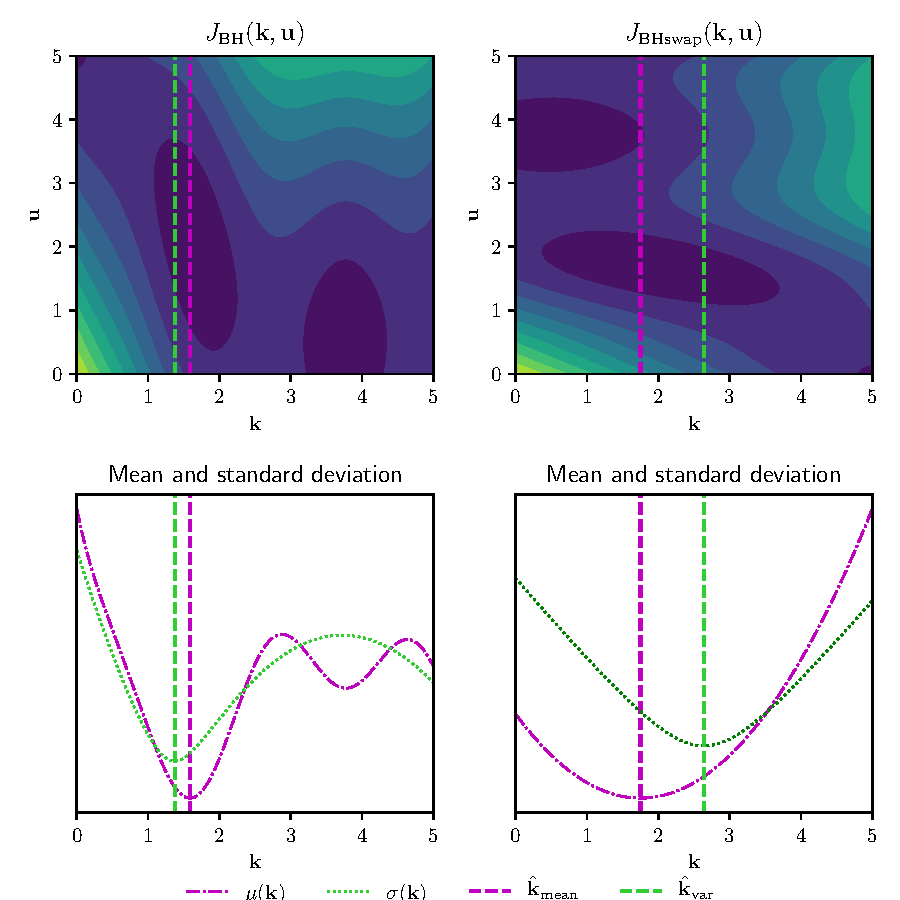
\includegraphics[width=\singlecolumnsize]{Figures/branin_side_moments_noscale.pdf}
  \caption{The left column concerns $\JBH$, while the right one deals with $\JBHS$. Contours of both functions are plotted on the top, and curves of  $\mu(\mathbf{k})$ and $\sigma(\mathbf{k})$ are shown on the bottom (respective scales are not displayed). Estimates $\hatkmean$ and $\hatkvar$ are plotted with the dashed line.}
\label{fig:branin_moments}
\end{figure*}
%\clearpage % Pour lisibilité dans le preview


The random variable $\mathbf{U}$ is assumed to be uniformly distributed over $\Uspace$.
%The definition and the estimation of $\kmean$ and $\kvar$ is pretty standard.  
The estimations are %$\mathbf{k}\mapsto \mu(\mathbf{k})$ and $\mathbf{k}\mapsto\sigma(\mathbf{k})$ 
based on a $1000 \times 1000$ regular grid over $\Kspace\times\Uspace$. Both cost functions are shown on the top of~Figure~\ref{fig:branin_moments}.


The left, (resp.\ right), column stands for $\JBH$ (resp.\ $\JBHS$).
Functions $\mu(\mathbf{k})$ and $\sigma(\mathbf{k})$ are drawn on the bottom row, respectively in purple and green. The corresponding minimisers $\hatkmean$ and $\hatkvar$ are also plotted.
On this figure, we can observe that $\hatkmean$ and $\hatkvar$ are close for $\JBH$, while being significantly different for $\JBHS$.
%\clearpage


Similarly, estimations of $\hatkmpe$ are depicted on Figure~\ref{fig:contours}. The top row shows the contours of both functions as well as the set of conditional minimisers $\{\mathbf{k}_{\mathbf{u}^i}\}_{1\leq i \leq N}$ in red, as defined in Eq.~\eqref{eq:conditional_minimiser}.
The bottom row presents three approximations of the density of minimisers: the histogram in grey (bin size selected using Freedman-Diaconis from~\cite{freedman_histogram_1981}), the result of a kernel density estimation (KDE) with Gaussian kernels in red (using Scott's rule from~\cite{scott_optimal_1979} for bandwidth selection), and the estimation by a Gaussian mixture, calculated with the EM algorithm. The number of Gaussians has been fixed to 3, a guess based on the general shape of the histogram. Respective estimations of $\hatkmpe$ are also depicted using dashed lines. 
\begin{figure}[!h]
  \centering
  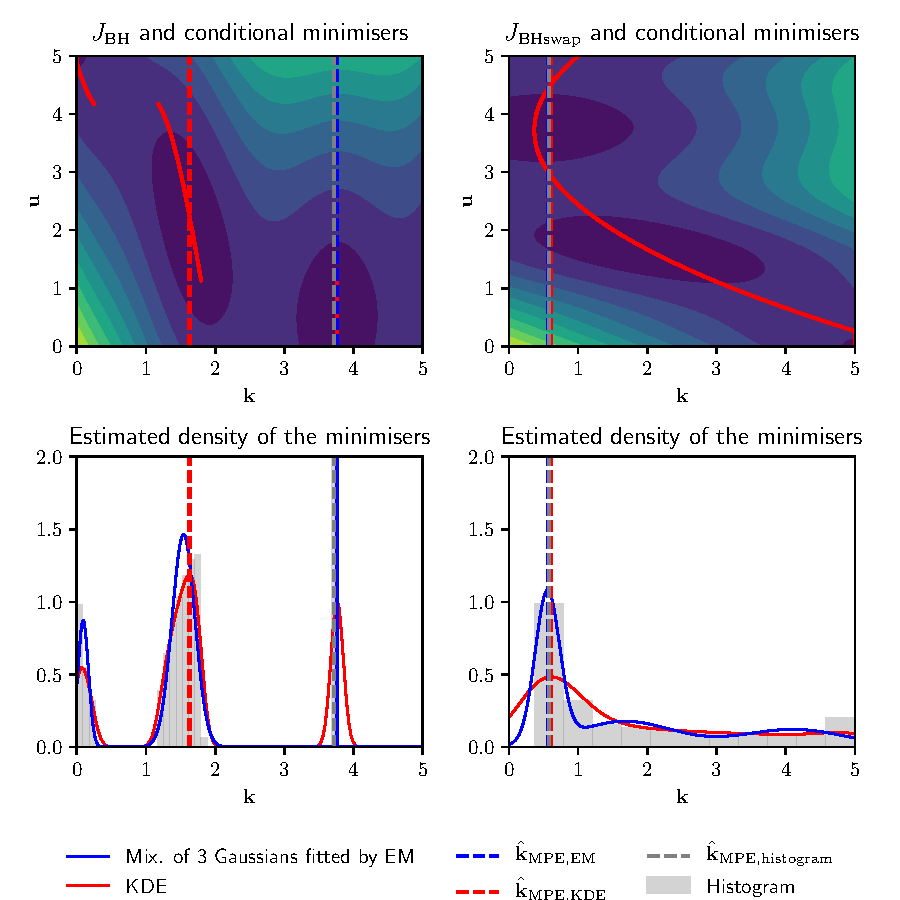
\includegraphics[width=\singlecolumnsize]{Figures/branin_side_66.pdf}
  \caption{Top Left:  $\JBH$ along with conditional minimisers in red. Bottom left: Estimated densities using KDE and EM algorithm and the histogram. The dashed lines indicate the MPE found using those methods. Right: Same quantities with $\JBHS$.}
\label{fig:contours}
\end{figure}

For $\JBHS$, we can observe that those three methods give consistent results, as $\hatkmpe {}_{,\mathrm{KDE}} =\hatkmpe {}_{,\mathrm{EM}}=\hatkmpe {}_{,\mathrm{histogram}}\approx 0.8$. This is not the case for $\JBH$: using Kernel density estimation (Gaussian), the estimation of $\kmpe$ is $\hatkmpe {}_{,\mathrm{KDE}} \approx 1.5$, while using the histogram and Gaussian mixture, $\hatkmpe {}_{,\mathrm{histogram}}=\hatkmpe {}_{,\mathrm{EM}}=3.8$.


This difference is explained by the accumulation of minimisers at this point: this challenges the assumption that $\mathbf{K}^*$ is continuous. As the density estimation techniques traditionally assume this continuity, the EM algorithm fits this using a normal distribution with a very small variance, while the KDE considers a sum of Gaussian kernels of constant bandwidth, located at the same point. This particular problem highlights an issue with $\kmpe$, as its estimation is possibly sensitive to the density approximation procedure.


Instead of just considering the optimal minimisers, we introduce a bit of leeway, and look for ``acceptably not optimal'' parameters.
 This slackness takes the form of a relaxation coefficient and its choice defines a new family of robust estimators, where each one of its member carries information on its robustness through this coefficient.
%This leads us to the definition of a new family of estimators, for which one can attribute a {\it level of robustness} \elise{je me rend bien compte que cette phrase est un peu bizarre ...mais bon c'est l'idee}


% ----------------------------------------------------------------------------


\section{Relative regret-based family of estimators}%A new family of robust estimators \elise{titre a revoir}}
\label{sec:relax_constraint}
\subsection{Relaxing the optimality constraint}
The density of minimisers has been estimated by optimising $\mathbf{k}\mapsto J(\mathbf{k},\mathbf{U}=\mathbf{u})$ over $\Kspace$ for different realisations of $\mathbf{u}$. Instead of focusing on optimal values, we propose to consider their {\it acceptable} neighbourhood in terms of performance of the cost function as well.
To do so, for each $\mathbf{u}$, $\mathbf{k}$ is deemed acceptable when  $J(\mathbf{k},\mathbf{U}=\mathbf{u}) \leq \alpha J^*(\mathbf{u})$, with $\alpha > 1$. 
%
%
In this context, for a given $\mathbf{k}$, the set $R_{\alpha}(\mathbf{k}) \subseteq \Uspace$ is defined as the set of $\mathbf{u}$, for which $\mathbf{k}$ is acceptable:
\begin{equation}
\label{eq:def_Ralpha}
R_{\alpha}(\mathbf{k}) = \left\{ \mathbf{u} \in \Uspace \mid J(\mathbf{k},\mathbf{U}=\mathbf{u}) \leq \alpha J^*(\mathbf{u}) \right\}
\end{equation}
Figure~\ref{fig:relax_tuto} details the successive steps for the construction of the set $R_{\alpha}$. First, the conditional minimisers are computed, as shown on the top plots. Afterwards, for a given level $\alpha=1.5$, the set of acceptable $\mathbf{k}$ can be identified for each $\mathbf{u} \in \Uspace$, as shown on the bottom left plot. Finally, the region $R_{\alpha}(\mathbf{k})$ is the subset of $\Uspace$ for which $\mathbf{k}$ is acceptable, as represented with a vertical slice on the bottom right plot.

% This notion of acceptability will be introduced later.
% Finally, for each $\mathbf{k}$, we will measure (with respect to $\Prob_{\mathbf{U}}$) the set of $\mathbf{u}$ within this acceptable neighbourhood. 


\begin{figure*}[!t]
\centering
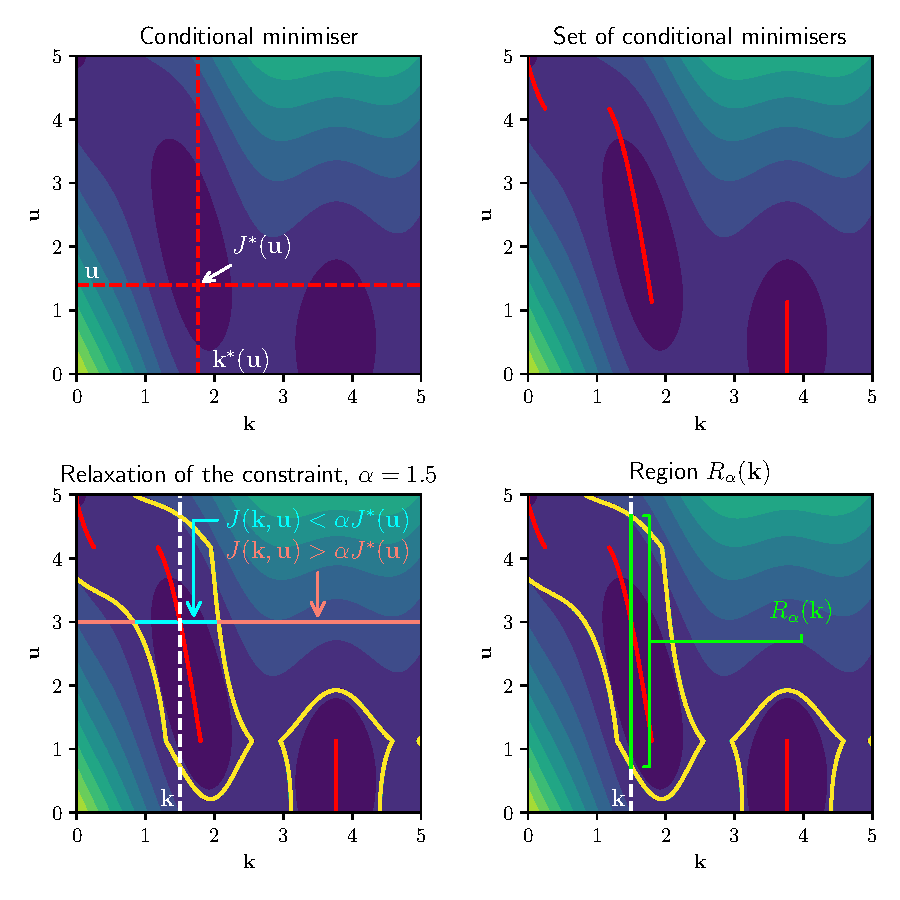
\includegraphics[width=\onehalfcolumn]{Figures/relaxation_tuto.pdf}
\caption{Principle of the relaxation of the constraint on $\JBH$, and illustration of $R_\alpha(\mathbf{k})$. Top plots: Computation of the conditional minimisers $\mathbf{k}^*(\mathbf{u})$. Top right plot: the set $(\mathbf{k}^*(\mathbf{u}),\mathbf{u})$ of conditional minimisers is represented in red. On the bottom left plot, for a relaxation $\alpha=1.5$, and $\mathbf{u}=3$, the acceptable $\mathbf{k}$ are in cyan, while the non-acceptable ones are in orange, while the frontier $\{(\mathbf{k}^*(\mathbf{u}),\mathbf{u}) \mid J^*(\mathbf{u}) = J(\mathbf{k},\mathbf{U}=\mathbf{u})\}$ is in yellow. On the bottom right plot, the set $R_{\alpha}(\mathbf{k})$ for $\alpha=1.5$ and $\mathbf{k}=1.5$ is in green.}
\label{fig:relax_tuto}
\end{figure*}

%In order to construct this region, we introduce a factor $\alpha \geq 1$, that will be multiplied to $J^*$:
%for a given $\mathbf{u}$, $\mathbf{k}$ is deemed acceptable if $J(\mathbf{k},\mathbf{u}) \leq \alpha J^*( \mathbf{u})$.
Introducing the random nature of $\mathbf{U}$, one can define $\Gamma_\alpha(\mathbf{k})$ as the probability that $\mathbf{k}$ is acceptable given $\alpha$:
\begin{equation}
  \label{eq:def_Gamma}
  \Gamma_\alpha(\mathbf{k}) = \Prob_{\mathbf{U}}\left[\mathbf{U} \in R_\alpha(\mathbf{k})\right] = \Prob_{\mathbf{U}}\left[J(\mathbf{k},\mathbf{U}) \leq 
    \alpha J^*(\mathbf{U}) \right]
\end{equation}
In other words, $\Gamma_{\alpha}(\mathbf{k})$ is the probability that $J(\mathbf{k},\mathbf{U})$ is between 
$J^*(\mathbf{U})$ and 
$\alpha J^*(\mathbf{U})$.


Noting that without relaxation, \textit{i.e.} when $\alpha$ is set to $1$, $\Gamma_1$ is non-zero if the set $\{\mathbf{u}\in\Uspace \mid J(\mathbf{k},\mathbf{U}=\mathbf{u}) = J^*(\mathbf{u})\}$ has non-zero measure with respect to $\Prob_{\mathbf{U}}$. It happens when the distribution of $\mathbf{K}^*$ presents atoms.

This can be linked to the definition of the distribution of the minimisers $\mathbf{K}^*$. For instance, if $\Kspace$ is a discrete set, we can rewrite $\Gamma_1$ as $\Gamma_1(\mathbf{k})=\Prob_{\mathbf{U}}\left[J(\mathbf{k},\mathbf{U}=\mathbf{u}) = J^*(\mathbf{U})\right] = \Prob_{\mathbf{U}}\left[\mathbf{k} = \mathbf{k}^*(\mathbf{U})\right]$ which is the probability mass function of $\mathbf{K}^*$.

The motivation behind this relaxation is to take into account the local behaviour of the function around the conditional minimisers.
For a given set of environmental conditions $\mathbf{u}$, if the function $\mathbf{k} \mapsto J(\mathbf{k},\mathbf{U}=\mathbf{u})$ is flat around its minimum $\mathbf{k}^*(\mathbf{u})$, then choosing  $\mathbf{k}^*(\mathbf{u}) + \epsilon$ (for a small $\epsilon$) will produce a value closer to the minimum than when the function has a high curvature.
In addition to that, relaxing the constraint using a multiplicative constant puts more weight on the values of $\mathbf{k}^*(\mathbf{u})$ when $J^*(\mathbf{u})$ is small.


The choice of the relaxation constant $\alpha$ can be made to ensure the existence of a parameter that is ``acceptable'' with a certain probability.
For instance, given that $J>0$, $\Gamma_{\alpha}(\mathbf{k})$ is increasing with respect to $\alpha$ for any $\mathbf{k}\in\Kspace$. We can then focus on the smallest value of $\alpha$ such that $\Gamma_\alpha$ reaches a certain level of confidence $p\in[0,1]$. This leads to the definition of $\checkap$
\begin{align}
  \checkap &= \inf\left\{ \alpha\geq 1 \mid \exists \checkkp \in \Kspace,\, \Gamma_{\alpha}(\checkkp) \geq p \right\} \nonumber \\
   &= \inf \left\{ \alpha \geq 1 \mid \max_{\mathbf{k}\in\Kspace} \Gamma_{\alpha}(\mathbf{k}) \geq p \right\}   \label{eq:def_alpha_check}
\end{align}
that is the smallest $\alpha$, such that there exists a particular $\checkkp \in \Kspace$ for which $J(\checkkp,\mathbf{U}) \leq \checkap J^*(\mathbf{U})$ with probability $p$.
$\{\mathbf{k}_p \text{ for } p \in [0;1] \}$ defines the relative-regret family of robust estimators (\RRE).
This formulation can be linked to the quantiles and Value-at-Risk of the random variable $\max_{\mathbf{k}} \{ J(\mathbf{k},\mathbf{U}) / J^*(\mathbf{U})\}$, that is a measure of risk usually applied in the financial sector (see~\cite{rockafellar_deviation_2002}). For different levels $p$, and thus different $\alpha_p$, Figure~\ref{fig:illu_alpha_p} shows examples of $\Gamma_{\alpha_p}$ for $\JBHS$. By definition, the associated $\mathbf{k}_p$ is then the first value for which $\Gamma_{\alpha_p}$ reaches $p$. We can see that changing the level $p$ shifts the maximiser of $\Gamma_{\alpha_p}$, and that for small $\alpha$, $\Gamma_{\alpha}(\mathbf{k}_1)$ is also very small. This indicates that $\mathbf{k}_1$ is located quite far from the conditional minimisers, and arise as a compromise when the relaxation is large enough.

\begin{figure}[!ht]
\centering
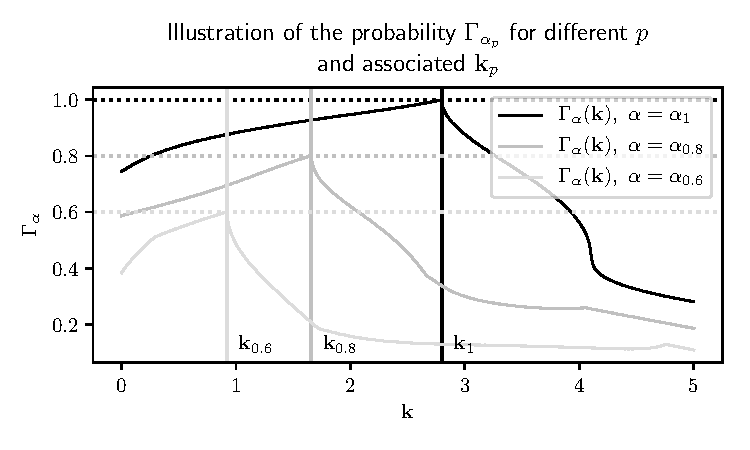
\includegraphics[width = \singlecolumnsize]{Figures/illu_alpha_p.pdf}
\caption{Illustration of the influence of different levels $p$ on $\Gamma_{\alpha_p}$ and on $\mathbf{k}_p$ for $\JBHS$}
\label{fig:illu_alpha_p}
\end{figure}



% For computational purpose, we can propose a loose upper bound on relevant values of $\alpha$ from Eq.~\eqref{eq:def_Ralpha}, provided that the maximum and minimum of $J$ is attained on $\Kspace\times\Uspace$. We have that for all $\mathbf{k}$, $\Prob_{\mathbf{U}}\left[J(\mathbf{k},\mathbf{U}) \leq \max_{\mathbf{k},\mathbf{u}} J\right]=1$, so
% \begin{equation}
%   \label{eq:upper_bound_alpha}
%   \alpha \geq \frac{\max_{(\mathbf{k},\mathbf{u})} J(\mathbf{k},\mathbf{u})}{\min_{(\mathbf{k},\mathbf{u})} J(\mathbf{k},\mathbf{u}) } \iff R_\alpha(\mathbf{k}) = 1 \quad \forall \mathbf{k}\in\Kspace
% \end{equation}

% In other words, this definition can be seen as the construction of the smallest confidence interval of level $p$:
% \begin{equation}
%  \label{eq:def_CI}
%  \Prob_{\mathbf{U}}\left[ \frac{J(\checkkp,\mathbf{U})}{J^*(\mathbf{U})}\in [1, \checka_p]\right] = p
%\end{equation}

By considering the particular case where $p=1$, a relation between $\checkk_1$ and $\checka_1$ can be derived, by using Eq.~\eqref{eq:def_alpha_check} and the strict positivity of the cost function:
\begin{equation}
  \label{eq:def_alpha1}
  \Prob_{\mathbf{U}}\left[\frac{J(\mathbf{k}_1,\mathbf{U})}{ J^*(\mathbf{U}) } \leq \checka_1\right]=1
\end{equation}
it follows then that 
\begin{equation}
  \label{eq:upper_bound_alpha_check}
  \checka_1 = \sup_{\mathbf{u}\in\Uspace} \frac{J(\mathbf{k}_1,\mathbf{U}=\mathbf{u})}{J^*(\mathbf{u})} =  \inf_{\mathbf{k}\in\Kspace} \left\{ \sup_{\mathbf{u}\in\Uspace} \frac{J(\mathbf{k},\mathbf{U}=\mathbf{u})}{J^*(\mathbf{u})} \right\} 
\end{equation}

This alternative definition of $\checka_1$ is useful to estimate it quickly whenever a grid over $\mathbb{K}\times\mathbb{U}$ has already been evaluated, thus avoiding multiple computations of $\Gamma_{\alpha}(\mathbf{k})$ until its maximum reaches $1$. From Eq.~\eqref{eq:upper_bound_alpha_check}, choosing a level of confidence equal to $1$ is then equivalent to looking for the worst-case scenario of the ratio ${J(\mathbf{k},\mathbf{U}=\mathbf{u})/J^*(\mathbf{u})}$. Therefore it may suffer from the same pitfall as the worst-case approach. As mentioned in the introduction, this is not suited for random variable with unbounded support as it may return over-conservative solution, provided that a solution exists in the first place.


$\checkap$ can be an indicator of the robustness of $\checkkp$.  
A high value of $\checka_1$ corresponds to a high ratio ${J(\mathbf{k},\mathbf{U}=\mathbf{u})/J^*(\mathbf{u})}$ for at least one particular $\mathbf{u}$. In that sense, $J(\checkk_1,\mathbf{U}=\mathbf{u})$ may be possibly very high.
More generally, for a fixed level of confidence $p$, $\checkap$ is the slackness needed to be able to reach the probability $p$. % So, in addition to the value of the estimate $\checkkp$, we have an indicator of the robustness associated.
We can then see that it is sensible to study jointly $p$, $\checkap$ and $\checkkp$.


\subsection{Choosing the relaxation coefficient}%Finding a balance between $p$ and $\checkap$}%Selection of a level of confidence}
\label{ssec:balance}

In order to choose the quantities introduced above, there are three choices: either fixing $p$, either fixing the maximal threshold $\alpha$, or looking for a compromise between $p$ and $\alpha$.
The most trivial way is to set $\alpha$, to find the couples of points $(\mathbf{k},\mathbf{u})$ verifying $J(\mathbf{k},\mathbf{U}=\mathbf{u}) \leq \alpha J^*(\mathbf{u})$, and then to estimate the probability $\Gamma_{\alpha}(\mathbf{k})$ defined in Eq.~\eqref{eq:def_Ralpha}.
For instance, when $N$ sampled values of $\mathbf{U}$: $\{\mathbf{u}^i\}_{1\leq i \leq N}$ are available, a possible estimator of $\Gamma_{\alpha}$ is
\begin{equation}
\hat{\Gamma}_{\alpha}(\mathbf{k}) = \frac{\mathrm{Card} \left\{\mathbf{u}^i \mid J(\mathbf{k},\mathbf{U}=\mathbf{u}^i) \leq \alpha J^*(\mathbf{u}^i)\right\}}{N}
\end{equation}
However, this may be a risky approach. Indeed if $\alpha$ is chosen too small, the resulting $\hat{p}=\max_{\mathbf{k}} \hat{\Gamma}_{\alpha}(\mathbf{k})$ will be also small, meaning that the cost function will have non acceptable values with high probability.

Similarly, if $p$ is fixed, the corresponding $\hat{\checka}_p$ is computed by searching for the smallest $\alpha$ satisfying $\max_{\mathbf{k}} \hat{\Gamma}_{\alpha}(\mathbf{k})=p$. Once again, if $\hat{\checka}_p$ is too large, the relaxation needed to get acceptable values with probability $p$ is very high, so the resulting estimation $\hat{\checkk}_p$ may not be relevant for the future application.

% \victor{chapeau car ici je parle de l'estimation en pratique}
Also, choosing $p=1$ is possible only if the sample space of $\mathbf{U}$ is bounded. An illustration of this flaw appears in the following simple problem:
\begin{align*}
  \label{eq:Jinfinite}
  \Kspace &= \Uspace = [0,\,+\infty[ \\
  J(\mathbf{k},\mathbf{U}=\mathbf{u}) &= \mathbf{u}(\mathbf{k}-\mathbf{u})^2 + 1 \\
  \mathbf{k}^*(\mathbf{u}) &= \mathbf{u} \\
  J^*(\mathbf{u}) &= 1
\end{align*}
In this case, for each $\mathbf{k}\in \Kspace$, $\lim_{\mathbf{u} \rightarrow + \infty} {J(\mathbf{k},\mathbf{U}=\mathbf{u})/J^*(\mathbf{u})} = + \infty$, so there is no $\mathbf{k}$ such that the ratio $J/J *$ can be bounded, hence $\alpha_1$ does not exist in this case.


Looking for a compromise between $p$ and $\alpha$ would be preferable. This could be achieved by studying $p \mapsto \checkap$, and particularly its slope.
If this curve presents a steep increase, the multiplicative constant $\checkap$ must be increased by a large amount in order to increase the probability $p$ by a small amount. Interesting couples $(p,\checkap)$ would then be the ones located before an abrupt increase of the slope of $p \mapsto \checkap$.

Another possibility is to model this compromise by the ratio $(p/\checkap)$, as it increases with respect to $p$ and decreases with respect to $\checka_p$. The level of confidence $p_{\mathrm{ratio}}$ is then defined as the maximiser of $p\mapsto p / \checka_p$.




% We are now going to compute and compare those estimators on the $\JBH$and $\JBHS$ function.



% ----------------------------------------------------------------------------
\subsection{Numerical Illustration}
\label{ssec:numerical_illustration}
% Numerical application}

In this Section, we will compare the different estimators introduced previously and summarised in Table~\ref{tab:RO_recap} on $\JBH$ and $\JBHS$.

\begin{table}[!h]
  \centering
\begin{tabular}{lrp{5cm}}
  \toprule
  Definition & Related quantities & Interpretation \\ \midrule
   $\argmin_{\mathbf{k}\in\Kspace} \Ex_{\mathbf{U}}\left[J(\mathbf{k},\mathbf{U})\right]$& $\kmean$ & Long run performances\\
   $\argmin_{\mathbf{k}\in\Kspace} \Var_{\mathbf{U}}\left[J(\mathbf{k},\mathbf{U})\right]$& $\kvar$  & Steady performances\\
   $\argmax_{\mathbf{k}\in\Kspace} p_{\mathbf{K}^*}(\mathbf{k})$ & $\kmpe$ & Most probable minimiser\\
    $\inf\left\{ \alpha \mid \exists \checkkp \in \Kspace,\, \Gamma_{\alpha}(\checkkp) \geq p \right\}$ & $(p, \checkkp,\checkap)$ & Acceptable values\newline with fixed probability $p$ \\
    $p_{\mathrm{ratio}} = \argmax p/\checkap$ & $(p_{\mathrm{ratio}}, \checkk_{\mathrm{ratio}}, \checka_{\mathrm{ratio}})$ & Maximal ratio of $p$ and $\checkap$ \\
  \bottomrule
\end{tabular}
\caption{Robust estimators, based on a cost function $J$}
\label{tab:RO_recap}
\end{table}


As stated before, we chose to model the uncertainties as a random variable uniformly distributed on $\Uspace$. The bounded nature of $\Uspace$ allows us to consider members of the \RRE{} up to a level of confidence $p=1$.
From now on, $\hatkmpe$ is estimated using KDE with Gaussian kernels.


The smallest estimated relaxation $\hat{\checka}_1$ and the corresponding $\hat{\checkk}_1$ has been computed for $\JBH$ and $\JBHS$, using a regular grid of $1000 \times 1000$ points on $\Kspace\times\Uspace$. The contour plots of those functions can be seen in the top plots of Figure~\ref{fig:contour_alpha}. The frontier corresponding to the couples of points $(\mathbf{k},\mathbf{u})$ verifying $\{J(\mathbf{k},\mathbf{U}=\mathbf{u}) = \alpha J^*(\mathbf{u})\}$ has been drawn on top of these contour plots, for $\alpha=\hat{\checka}_1$ and an arbitrary $\alpha=1.5<\hat{\checka}_1$ to illustrate the effect of the acceptable region when the relaxation $\alpha$ changes. 
On the bottom plots, the curves $\mathbf{k}\mapsto \hat{\Gamma}_{\alpha}(\mathbf{k})$ for $\alpha=\hat{\checka}_1$ and $\alpha=1.5$ along with the histograms of the minimisers are represented.


One can notice that the relaxation allows us to avoid the issue brought by the accumulation of the minimisers of $\JBH$ at $3.8$, as opposed to the MPE and its dependence on the estimation procedure of the distribution.

\begin{figure*}[!ht]
  \centering
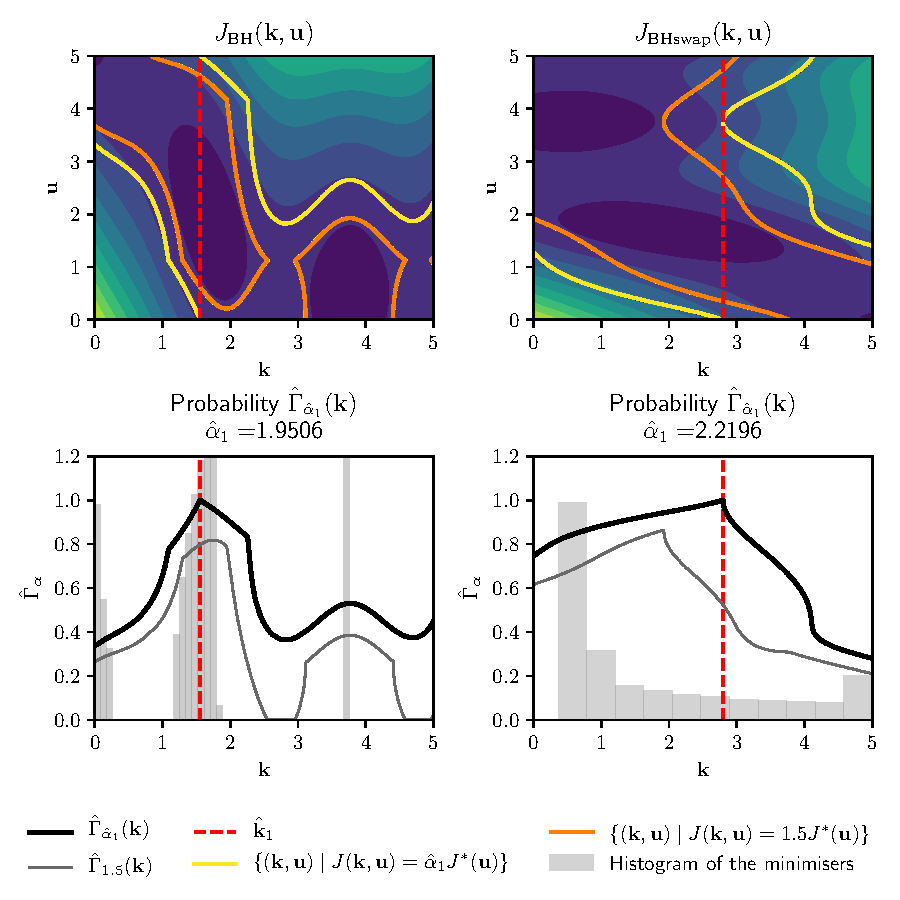
\includegraphics[width=\onehalfcolumn]{Figures/branin_side_66_relax_gamma_both.pdf}
\caption{Top: $\JBH$ and $\JBHS$ contours. The thick yellow lines are the boundaries of the acceptable region defined for $\hat{\checka}_1$, the thick orange are for $\alpha=1.5$. The red dashed line is the estimation $\hat{\checkk}_1$. Bottom: $\hat{\Gamma}_{\alpha}$ for $\alpha = 1.5$ and $\alpha=\hat{\checka}_1$, and estimated density of the minimisers.}
\label{fig:contour_alpha}
\end{figure*}

% For the $\JBH$ function (left), the $\hat{\checka}_1$, $\hatkmean$ and $\hatkvar$ are quite close, so naturally we would expect a robust estimate to be significantly close to those values. $\hat{\checkk}_1$ supports this intuition, and appears to be very close to $\hatkmean$. 
%Concerning the $\JBHS$ function (right), $\hat{\checkk}_1$ appears to be closer to $\hatkvar$ this time.s

In order to choose a satisfying level of confidence $p$, we are going to study $p\mapsto \hat{\checka}_p$ and $p\mapsto p/\hat{\checka}_p$, as described in Section~\ref{ssec:balance}.

 The plot of $p\mapsto \hat{\checka}_p$ for $\JBH$ on Figure~\ref{fig:ratio_BH} shows what seems to be a piecewise linear behaviour. The last change of slope, \textit{i.e.} for $p\approx 0.9$ corresponds to a local maximum of the ratio, while the first change of slope at $\hat{p}_{\mathrm{ratio}}=0.654$ corresponds to the global maximum of the ratio. The \RRE{} will then be evaluated for both of these values, as well as $p=1$ for reference.
 
 \begin{figure}[!ht]
   \centering
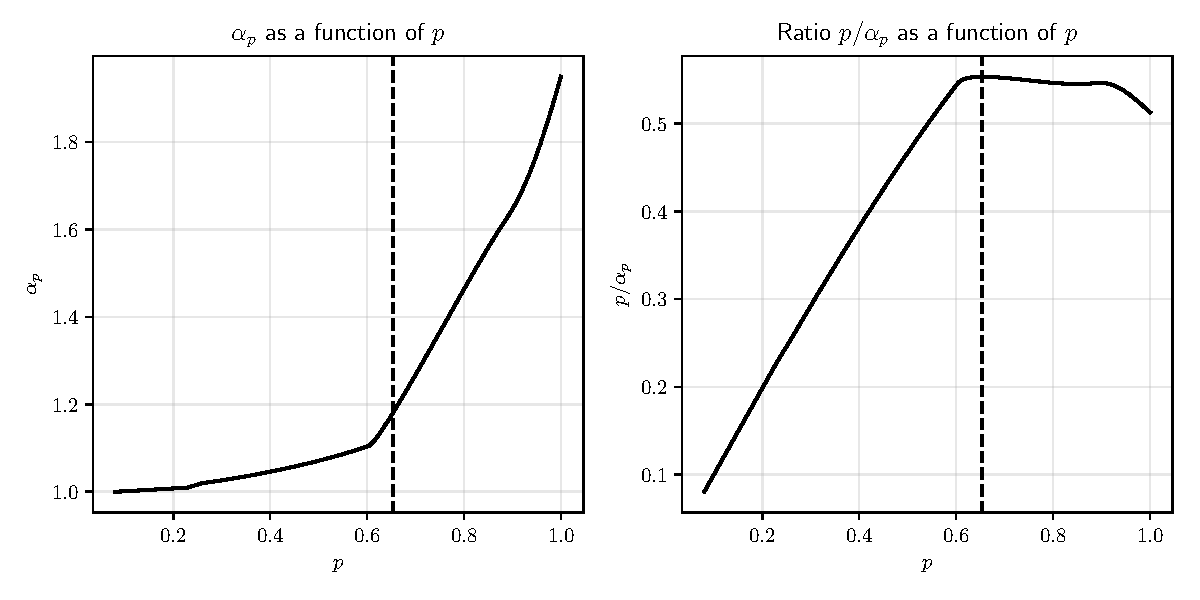
\includegraphics[width=\onehalfcolumn]{Figures/alpha_p_BH.pdf}
\caption{Evolution of the couples $(p,\checkap)$ and corresponding ratio $p/\checkap$ for $\JBH$. The dashed line indicates the level $p$ associated with the highest ratio}
\label{fig:ratio_BH}
\end{figure}


 For $\JBH$, the numerical values of the robust estimators can be found in Table~\ref{tab:recap_estimates_branin}. For this particular problem, the different estimates are close to each other.
 
% \begin{table*}[!ht]
% \centering
% \caption{Estimation performed for $\JBH$, sorted by value}
% \label{tab:recap_estimates_branin}
% \begin{tabular}{lr}
% \toprule
% Estimate & Value \\ \midrule
% $\hatkvar$ & 1.371 \\ 
% $\kest_p,~p=1$ & 1.557 \\ 
% $\hatkmean$ & 1.587 \\ 
%   $\hatkmpe$ & 1.628 \\
%   $\kest_{\mathrm{ratio}},~\hat{p}_{\mathrm{ratio}}=0.654$ & 1.637 \\
% $\kest_p,~p=0.95$ & 1.672 \\ \bottomrule
% \end{tabular}
% \end{table*}
\begin{table}[!h]
  \centering
\caption{Estimation performed for $\JBH$, sorted by value}
\begin{tabular}{lr}
  \toprule
Estimate & Value \\ \midrule
$\hatkvar$ & 1.371 \\ 
$\kest_{p},~p=1$ & 1.557 \\ 
$\hatkmean$ & 1.587 \\ 
$\kest_{\mathrm{MPE}}$ & 1.628 \\ 
$\kest_{\mathrm{ratio}},~\hat{p}_{\mathrm{ratio}}=0.654$ & 1.637 \\ 
$\kest_p,~p=0.90$ & 1.797 \\  \bottomrule
\end{tabular}
\label{tab:recap_estimates_branin}
\end{table}
Practically speaking, in order to compare the effective values taken by the objective function given an estimate $\kest$ we are going to consider the functions $\mathbf{u} \mapsto J(\kest,\mathbf{U}=\mathbf{u})$, that we will call ``profiles of $\kest$''. Those profiles are well suited for the representation of the cost function for an estimate $\kest$ fixed as the uncertain variable is modelled with a 1D uniform random variable.

For $\JBH$, the curves are plotted in Figure~\ref{fig:profiles_branin}.

\begin{figure*}[!h]
  \centering
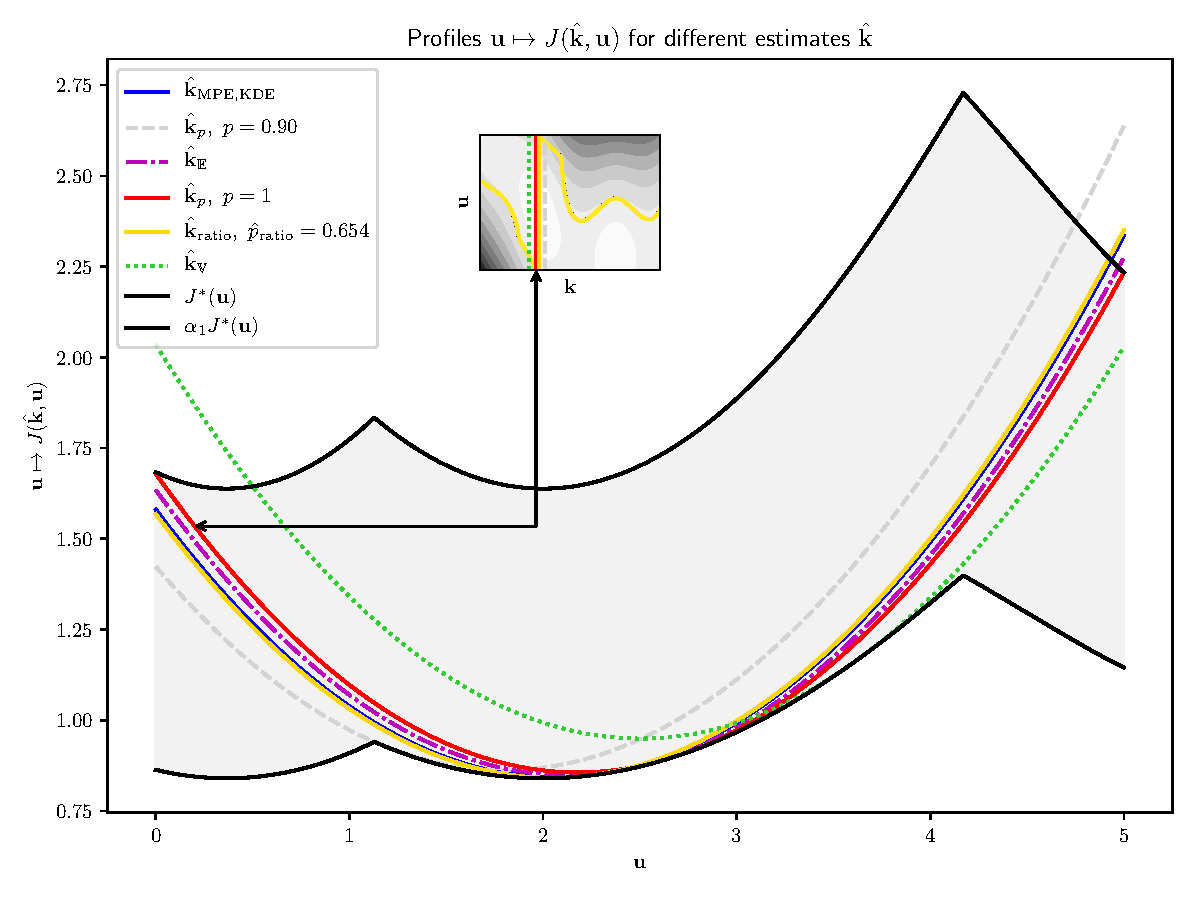
\includegraphics[width=\onehalfcolumn]{Figures/profile_BH.pdf}
\caption{Profiles of the different estimates for $\JBH$, corresponding to the vertical cross sections of the contour. The shaded region corresponds to the interval $[J^*(\mathbf{u}), \hat{\checka}_1 J^*(\mathbf{u})]$. The profiles of $\kest_{\mathrm{MPE}}$ and $\kest_{\mathrm{ratio}}$ coincide in this case}
\label{fig:profiles_branin}
\end{figure*}

By construction, the profile of $\hat{\checkk}_1$ is always within the shaded region, corresponding to $[J^*(\mathbf{u}), \hat{\checka}_1 J^*(\mathbf{u})]$. The profile of $\hatkmean$ in contrast, exceeds $\hat{\checka}_1 J^*(\mathbf{u})$ for $\mathbf{u}$ close to $5$, while the profile of $\hatkvar$ does it for $\mathbf{u}$ close to $0$. Except for $\hatkvar$, the different estimators give somewhat comparable results.


By contrast, $\JBHS$ will show a different behaviour as Figure~\ref{fig:ratio_BHs} provides the plots of $p\mapsto \hat{\checka}_p$ and $p\mapsto p/\hat{\checka}_p$.

\begin{figure}[!h]
  \centering
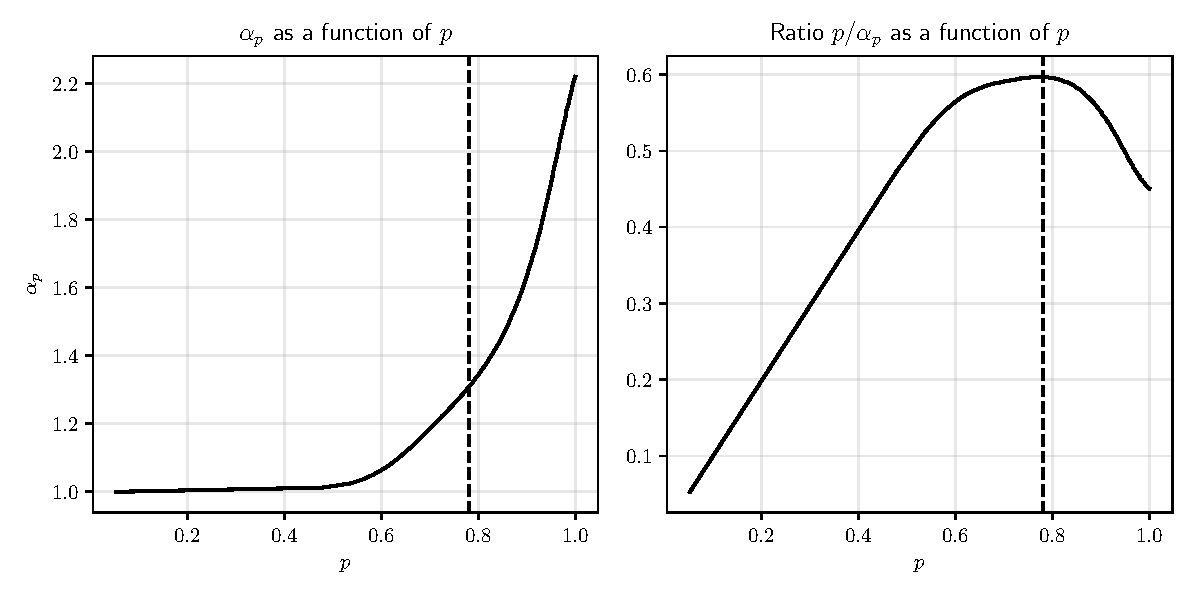
\includegraphics[width=\onehalfcolumn]{Figures/alpha_p_BHs.pdf}
\caption{Evolution of the couples $(p,\checkap)$ and corresponding ratio $p/\checkap$ for $\JBHS$. The dashed line indicates the level $p$ associated with the highest ratio}
\label{fig:ratio_BHs}
\end{figure}

Compared to the similar plots for $\JBH$ in Figure~\ref{fig:ratio_BH}, $\hat{\checka}_p$ exhibits a smoother behaviour for $\JBHS$ as no abrupt change of slope is easily discernable and the ratio presents a unique maximum for $\hat{p}_{\mathrm{ratio}}=0.766$. The numerical values of the estimations $\kest$ presented in Table~\ref{tab:recap_estimates_BHs} show that, contrary to $\JBH$, the calibrated values are more spread over $\Kspace$.

\begin{table}[!h]
\centering
\caption{Estimations performed for $\JBHS$, sorted by value}
\label{tab:recap_estimates_BHs}
\begin{tabular}{lr} \toprule
Estimate & Value \\ \midrule
$\kest_{\mathrm{MPE}}$ & 0.606 \\ 
$\kest_{\mathrm{ratio}},~ \hat{p}_{\mathrm{ratio}}=0.766$ & 1.537 \\ 
$\hatkmean$ & 1.752 \\ 
$\hatkvar$ & 2.638 \\ 
$\kest_1,~p=1$ & 2.798   \\ \bottomrule
\end{tabular}
\end{table}


Profiles of the different estimates of $\JBHS$ are shown in Figure~\ref{fig:profiles_branin_switch}.

\begin{figure*}[!h]
  \centering
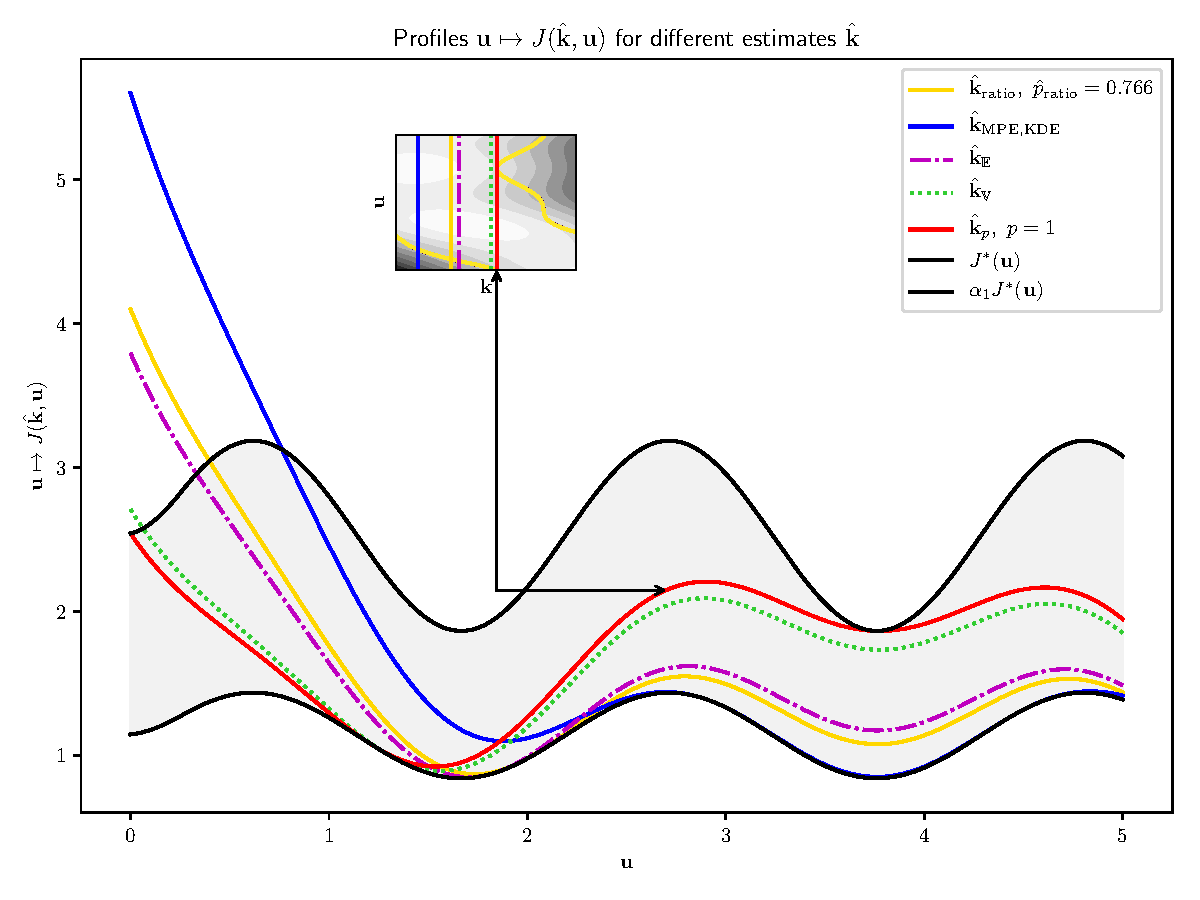
\includegraphics[width=\onehalfcolumn]{Figures/profile_BHs.pdf}
\caption{Profiles of the different estimates for $\JBHS$. Those profiles are the vertical cross sections of the contours above. The shaded region corresponds to the interval $[J^*(\mathbf{u}), \hat{\checka}_1 J^*(\mathbf{u})]$}
\label{fig:profiles_branin_switch}
\end{figure*}

In this case, $\hatkmpe$, $\hatkmean$ and $\hat{\checkk}_{\mathrm{ratio}}$ present a similar behaviour.
They perform very well for $\mathbf{u}>2$, especially for $\hatkmpe$ which is very close to the minimal value; however for $\mathbf{u}<2$, they produce high values of the function.
The performances of $\hat{\checkk}_1$ are closer to the performances of $\hatkvar$ for this function, but it performs worse than $\hatkmean$ and $\hatkvar$ for $\mathbf{u}>2$, even though its range is designed to stay within the interval $[J^*(\mathbf{u}); \hat{\checka}_1 J^*(\mathbf{u})]$.



We have seen how some classical robust estimators and the \RRE{} behave on two different analytical problems. In addition to the usual levels of confidence such as 90\% and 95\%, one can also settle for an ad-hoc compromise, where $p$ maximizes the ratio $p/\alpha_p$. When the sample space of $\mathbf{U}$ is bounded, a conservative solution is to set $p=1$.
We are now going to see how can robust minimisation is applied on the calibration of a numerical model.
% ----------------------------------------------------------------------------

% ----------------------------------------------------------------------------
\section{Robust calibration of a numerical model}
\label{sec:SWE_application}
% ----------------------------------------------------------------------------

\subsection{Calibration of a toy numerical model}
 We will follow the approach described in~\cite{kennedy_bayesian_2001} in order to establish the function $\mathcal{G}$ described in the first section in Eq.~\eqref{eq:def_cost_fun}, and the resulting cost function $J$.
 
 The calibration of a numerical model is usually based on the comparison between the numerical model and some observations, during a fixed time interval $[0, T]$ called assimilation window.
 The modelled physical system can be seen as a map from $\Uspace$ to $\mathbb{Y}$, the space of observations, denoted as $\mathcal{M}^o : \mathbf{u}\mapsto \mathcal{M}^o(\mathbf{u})$, where $\mathbf{u}\in\Uspace$ is an input representing some environmental conditions. The observation mentioned above is the output of the physical system during the time-window, and is denoted by $\mathcal{M}^o(\mathbf{u}^{\mathrm{true}}) \in \mathbb{Y}$, where $\mathbf{u}^{\mathrm{true}} \in \Uspace$ is unknown.

 
In addition of $\mathbf{u}$, the numerical model $\mathcal{M}$ depends on some other input $\mathbf{k}\in\Kspace$. This additional parametrization comes usually from the successive simplifications needed to implement a numerical model of the observed physical system. $\mathbf{k}$ needs to be calibrated accordingly, so that the numerical model can be used to predict the behaviour of the physical system under different operating conditions.

The misfit $\mathcal{G}$ is defined as the difference between the numerical model and the observation. Choosing a squared norm, the cost function $J$ defined in Eq.~\eqref{eq:def_cost_fun} is
\begin{equation}
J(\mathbf{k},\mathbf{U}=\mathbf{u}) = \frac12 \| \mathcal{G}(\mathbf{k},\mathbf{u}) \|^2 = \frac12 \|\mathcal{M}(\mathbf{k},\mathbf{u}) - \mathcal{M}^{o}(\mathbf{u}^{\mathrm{true}}) \|^2
\end{equation}
\subsection{The Shallow Water equations}

The model to calibrate is an implementation of the 1D Shallow Water equations, described in Eq.~\eqref{eq:SWE_equations}, where $h$ is the height of the water column, $q$ the discharge, and $z$ the bathymetry, while $g$ is the usual gravitation constant. The parameter to calibrate $\mathbf{k}$ is the quadratic friction term, proportional to the square of the inverse of Manning-Strickler coefficient. The environmental parameter $\mathbf{u}$ is the amplitude of a sine wave of period $1/\omega_0$. The domain of those two parameters are $\Kspace = [0.0, 1.3]$ and $\Uspace = [0.5, 0.7]$.


\begin{align}
  \label{eq:SWE_equations}
  \left\{
    \begin{array}{rl}
      \partial_t h + \partial_x q &= 0 \\
      \partial_t q + \partial_x \left(\frac{q^2}{h} + \frac{g}{2}h^2\right) &= - gh\partial_x z - \mathbf{k}q |q|h^{-7/3} \\
      h(0, t) &= 20.0 + 3\cdot \sin \left(\frac{2\pi t}{2}\right) + 1.5\cdot \mathbf{u} \cdot \sin\left(\frac{2 \pi t}{\omega_0}\right)\\
      \partial_x q(0, t) &= 0
      \end{array}
  \right.
\end{align}

These equations are integrated using a finite-volume scheme on a discretized domain $[0, L]$, up to a time $T$. The output of the computer code is the sea surface height $h$, on the center of all the volumes and at all the time-steps, that will be denoted $\mathcal{M}(\mathbf{k},\mathbf{u};\, \omega_0=1.0)$.
In this setting, the random variable $\mathbf{U}$ is uniformly distributed on $\Uspace$.

To generate the observation, we set $\mathbf{u}^{\mathrm{true}}=2/3$, and define $\mathcal{M}^o$ based on the computer model $\mathcal{M}$, such that $\mathcal{M}^o(\mathbf{u}^{\mathrm{true}}) = \mathcal{M}(\mathbf{k}^{\mathrm{true}}, \mathbf{u}^{\mathrm{true}}; \, \omega_0 = 0.999)$. $\omega_0$  
represents here the uncontrollable error between the observations and the numerical model and will now be omitted systematically in the notation.

The true value of the bottom friction $\mathbf{k}^{\mathrm{true}} = (k_1^{\mathrm{true}}, k_2^{\mathrm{true}},\dots, k_{N_\mathrm{vol}}^{\mathrm{true}})$ is not constant over the whole domain, and is defined as
\begin{equation*}
{k}^{\mathrm{true}}_i = 0.2\cdot \left(1 + \sin\left(\frac{2 \pi x_i}{L}\right)\right)
\end{equation*}
where $x_i$ is the center of the $i$-th volume. The two sources of systematic errors are the one-dimensionality of $\Kspace$, and $\omega_0$.
Given this setting, there exists no couple $(\mathbf{k},\mathbf{u})\in\Kspace \times \Uspace$ reproducing exactly the observations, thus the cost function will always be strictly positive.

\subsection{Computation of the robust estimates}
As the numerical model is expensive to run, it has first been evaluated on a relatively small regular grid covering $\Kspace \times \Uspace$, and a metamodel based on Gaussian processes is constructed using those initial evaluations. In order to better capture the locus of the conditional minimisers $\{(\mathbf{k}^*(\mathbf{u}), \mathbf{u}) \mid \mathbf{u} \in \Uspace \}$, we select points maximising the PEI criterion~\citep{ginsbourger_bayesian_2014,bossek_learning_2015} in order to add points to the design that improve the metamodel accuracy close to the conditional minimisers.
Afterwards, a bigger regular grid is evaluated by the metamodel once the design space has been sufficiently explored, and these computations are used to calibrate the model.

The different steps of the estimation are illustrated Figure~\ref{fig:estimation_swe}, where the top plot shows the contour plot of $J$, with the conditional minimisers and the \RRE{} of level $p=1$. On the middle plot are shown the conditional moments, $\hatkmean$ and $\hatkvar$ and the estimated density of the minimisers. At the bottom of the Figure, $\hat{\Gamma}_{\alpha_p}$ are represented for different levels $p$. As $\Uspace$ is bounded, $p=1$ is attainable, and $\kest_1$ is evaluated.

\begin{figure}[!h]
\centering
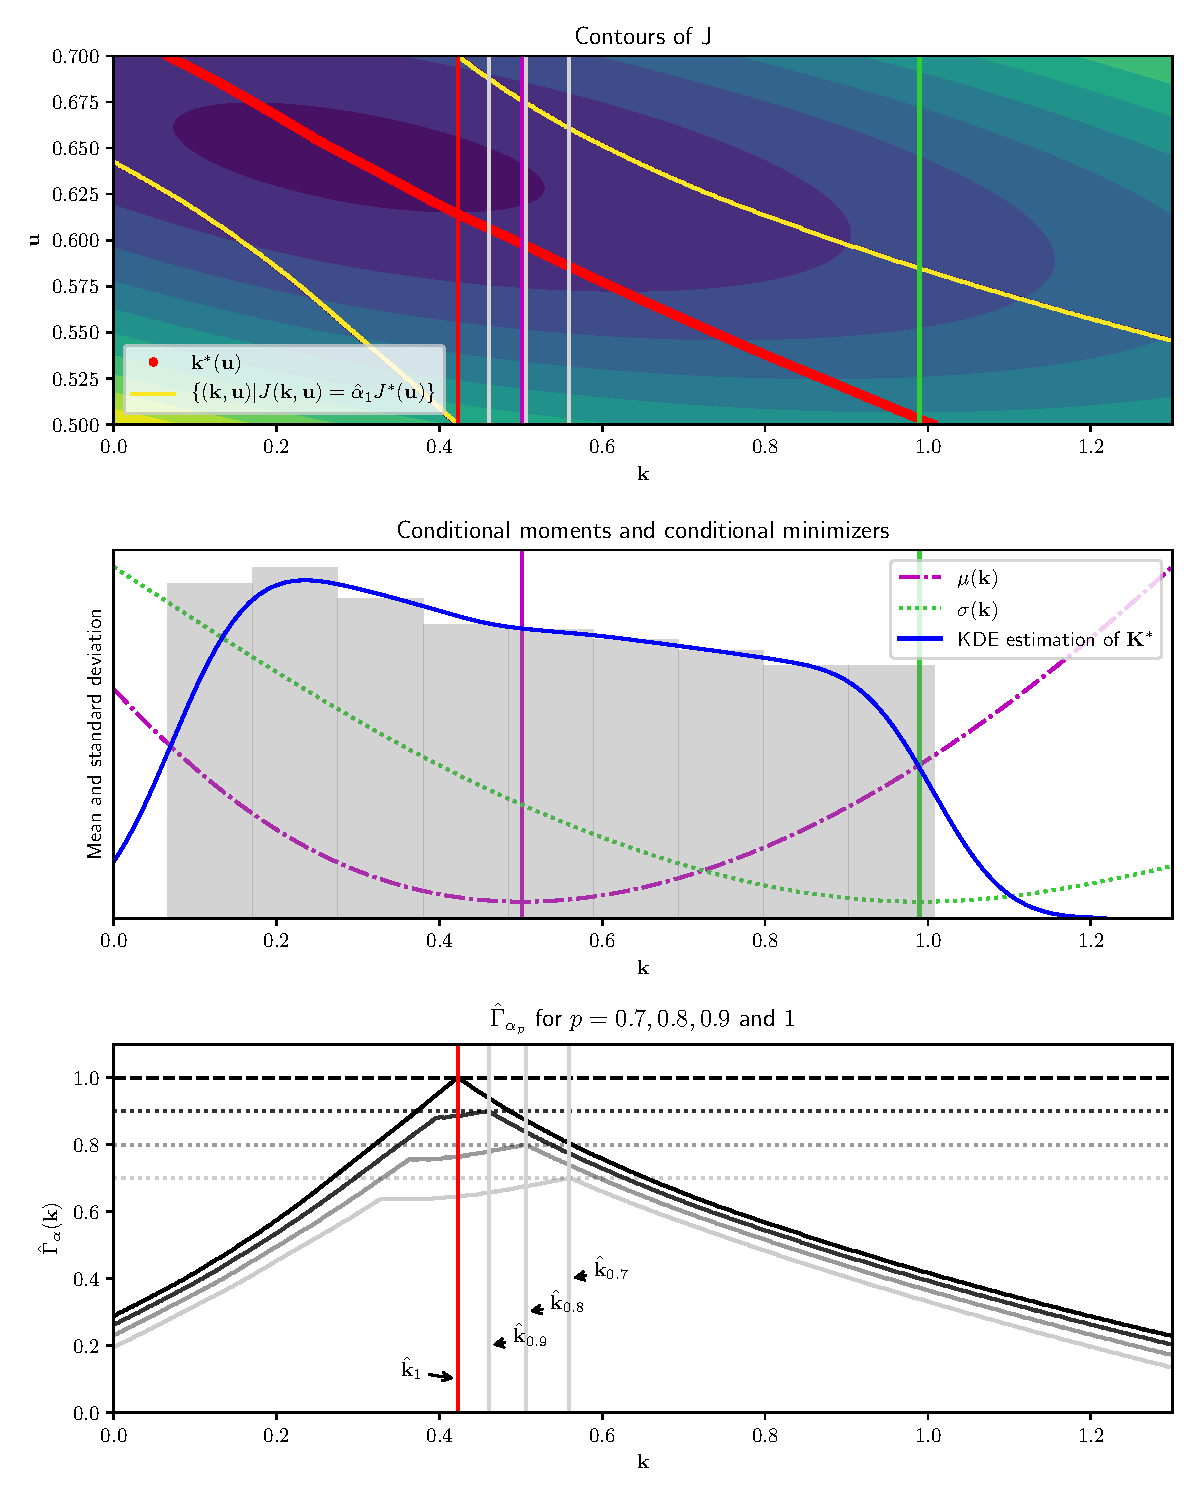
\includegraphics[width=\singlecolumnsize]{Figures/RobustSWEmis_plots.pdf}
\caption{Procedure of robust calibration for the shallow water problem. Top: contours of $J$, conditional minimisers and $\{(\mathbf{k},\mathbf{U}=\mathbf{u}) | J(\mathbf{k},\mathbf{u}) = \hat{\alpha}_1 J^*(\mathbf{u})\}$. Middle: Conditional moments and histogram and KDE of the conditional minimisers. Bottom: $\hat{\Gamma}_{\alpha_p}$ for different levels $p$}
\label{fig:estimation_swe}
\end{figure}

We can see that the different estimations seem less problematic for this problem than for the analytical examples shown in Section~\ref{ssec:numerical_illustration}, as everything appears to be very smooth and unimodal.

Looking at $p\mapsto \alpha_p$ and $p\mapsto p/\alpha_p$ on Figure~\ref{fig:alpha_p_SWE}, we can see that $\alpha_p$ evolves almost linearly for $p>0.5$, and that the ratio $p/\alpha_p$ is monotonically increasing, so that the maximal ratio is found for $p=1$.  

\begin{figure}[!h]
  \centering
  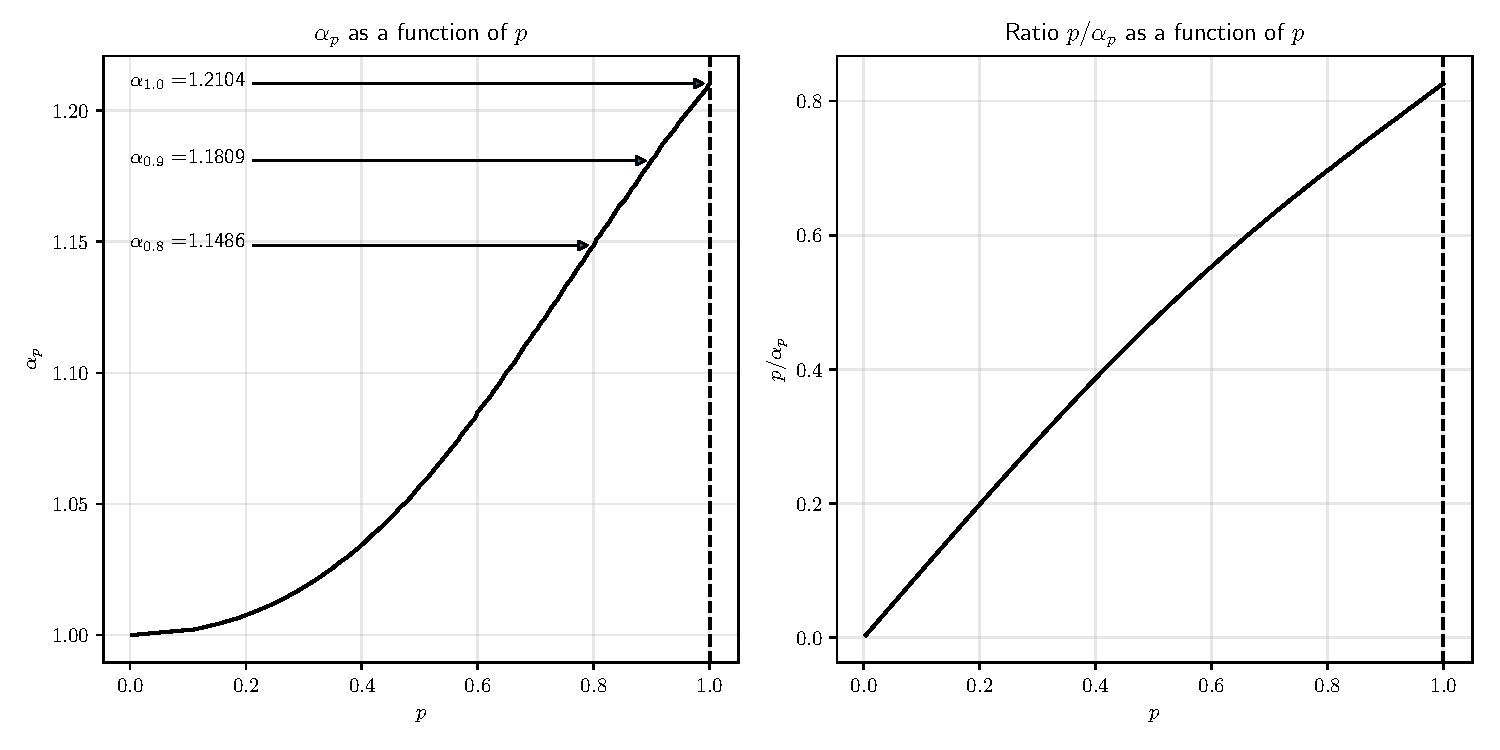
\includegraphics[width=\onehalfcolumn]{Figures/alpha_SWE}
  \caption{Evolution of $\alpha_p$ for different levels $p$, and ratio, for the shallow water problem}
\label{fig:alpha_p_SWE}
\end{figure}

The different estimates take a wide range of values, as seen on Table~\ref{tab:recap_estimates_metaSWE}, from $0.249$ to almost $1.0$, while $k_i^{\mathrm{true}} \in [0, 0.4]$ for $1\leq i \leq N_{\mathrm{vol}}$. It can be noted that the calibration may lead to values outside the range given by the true ones. This can be interpreted as the fact that the calibration look to compensate for errors on $\omega_0$. 
As a basis for comparison, the global minimiser of $J$ over $\Kspace \times \Uspace$ has also been computed, and $\kest_{\mathrm{global}}$ is then obtained by discarding the $\mathbf{u}$ value.



\begin{table}[!h]
\centering
\caption{Calibrated values of $\mathbf{k}$ according to different criteria, for the shallow water problem}
\begin{tabular}{lr} \toprule
Estimate & Value \\ \midrule
$\hatkmpe$ & 0.249 \\
$\kest_{\mathrm{global}}$ & 0.290 \\
$\hatkp,~p=1$ & 0.423 \\ 
$\hatkp,~p=0.90$ & 0.458 \\ 
$\hatkmean$ & 0.501 \\ 
$\hatkp,~p=0.80$ & 0.505 \\ 
$\hatkp,~p=0.70$ & 0.560 \\ 
$\hatkvar$ & 0.990\\ \bottomrule
\end{tabular}
\label{tab:recap_estimates_metaSWE}
\end{table}

Similarly as for $\JBH$ and $\JBHS$, the profiles are depicted Figure~\ref{fig:profiles_swe}.
\begin{figure}[!h]
  \centering
  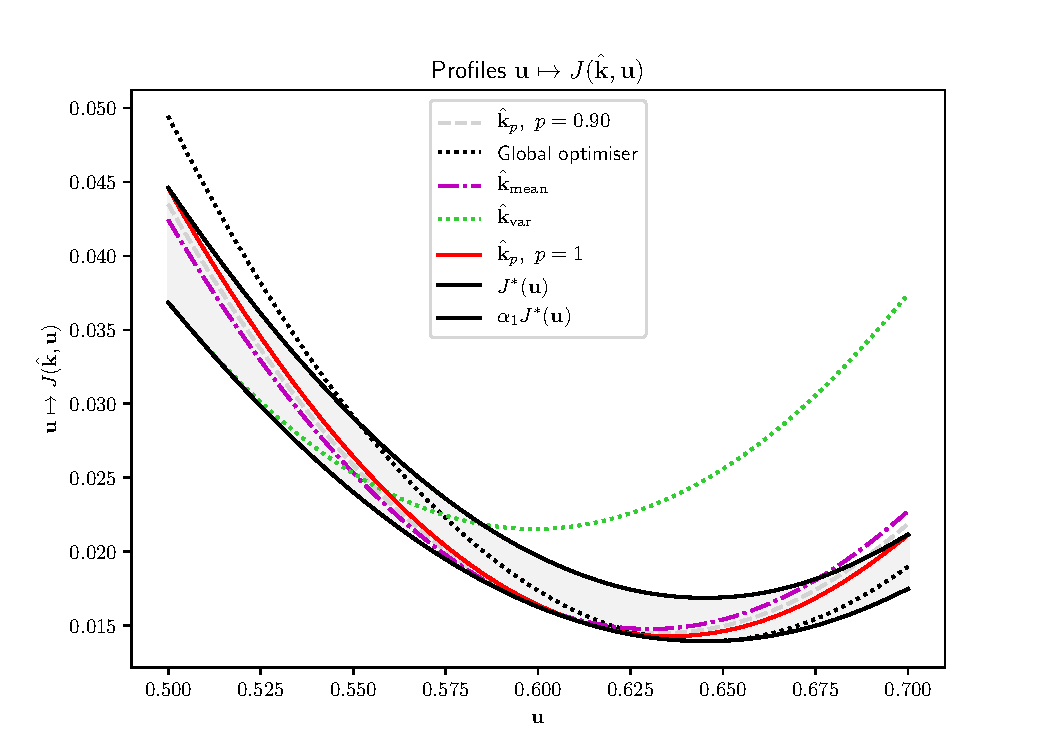
\includegraphics[width=\onehalfcolumn]{Figures/profile_swe}
  \caption{Profiles for the calibration problem, for the shallow water case}
\label{fig:profiles_swe}
\end{figure}


We can see that the performances of $\kest_1$ and $\hatkmean$ are very similar, but $\kest_1$ has better performances when $\mathbf{u} > 0.6$. When comparing with the global optimiser $\kest_{\mathrm{global}}$, $\kest_1$ performs better when $\mathbf{u}<0.625$, so more than half of the time.
We are now going to compare how well some of those calibrated values compare in a forecast context.


\subsection{Assessing the quality of the forecast of the calibrated model}
For the calibration, the model has been integrated on a time-period $[0, T]$, called assimilation window, and have been compared with the observation of the sea water height on the same time-period.
We now want to compare the quality of the different forecasts originating from different calibrated bottom frictions.
Those forecasts result from the integration of the numerical model between the time $T$ and a time $T_{\mathrm{pred}}$: the forecast window.

Given the probabilistic nature of the environmental conditions $\mathbf{U}$, the forecasts will also be probabilistic. We will then compare $\mathcal{M}_{\mathrm{pred}}^o(\mathbf{U})$ and $\mathcal{M}_{\mathrm{pred}}(\mathbf{k},\mathbf{U})$, that are the observation, and the numerical model on the forecast window for a calibrated $\mathbf{k}$.

Two metrics will be computed: the squared forecast error, and the Continuous Ranked Probability Score (CRPS)~\citep{gneiting_probabilistic_2014}. The parameters satisfying a robust criterion that are compared are the minimiser of the expectation $\hatkmean$, the minimiser of the variance $\hatkvar$ and the relative regret of level $p=1$, $\kest_1$ as described in the previous section.
We will also feature the global minimiser $\kest_{\mathrm{global}}$, and the conditional minimisers $\kest^*(\mathbf{u}^i)$ where the chosen environmental variables are $\{\mathbf{u}^i\}_{1\leq i \leq 4} = \{0.5, 0.55, 0.65, 0.7\}$. Those values, even though they do not meet a robustness criterion, are introduced in order to have a more precise idea on the possible performances of a deterministic version of the calibration problem.
The conditional minimiser $\kest^*(0.6)$ has been omitted as it results in a value very similar to the minimum of the expectation.

\subsubsection{Squared forecast error}
A first simple approach to measure the forecast quality is to take the squared difference between the numerical model and the observation for two samples of $\mathbf{U}$.
Given two environmental conditions $\mathbf{u}$ and $\mathbf{u}'\in \Uspace$, the former used to run the computer simulation and the latter to generate the observations, the squared forecast error for the parameter $\mathbf{k}$ is

\begin{equation}
\label{eq:squared_forecast_error}
S_{\mathrm{pred}}(\mathbf{k},\mathbf{u},\mathbf{u}') = \left(\mathcal{M}_{\mathrm{pred}}(\mathbf{k},\mathbf{u}) - \mathcal{M}^{o}_{\mathrm{pred}}(\mathbf{u}')\right)^2
\end{equation}

Averaging over both $\mathbf{u}$ and $\mathbf{u}'$ defines the mean squared forecast error, defined on every point of the spatial domain, and at every time-steps. This can be done using a Monte-Carlo approximation. As $\mathbf{u}$ and $\mathbf{u}'$ are i.i.d., assuming that we have a set of samples $\{\mathbf{u}^i\}_{1\leq i \leq N_{\mathbf{u}}}$, the squared forecast error can then be approximated:

\begin{equation}
  \label{eq:squared_forecast_error_averaged}
  S(\mathbf{k}) = \frac{1}{N_{\mathbf{u}}^2 }\sum_{i=1}^{N_{\mathbf{u}}}\sum_{j=1}^{N_{\mathbf{u}}} S_{\mathrm{pred}}(\mathbf{k},\mathbf{u}^i,\mathbf{u}^j) = \frac{1}{N_{\mathbf{u}}^2 }\sum_{i=1}^{N_{\mathbf{u}}}\sum_{j=1}^{N_{\mathbf{u}}}  \left(\mathcal{M}_{\mathrm{pred}}(\mathbf{k},\mathbf{u}^i) - \mathcal{M}^{o}_{\mathrm{pred}}(\mathbf{u}^j)\right)^2
\end{equation}

The mean squared forecast error averaged over the whole space and over all the time-steps gives an indication on the overall prediction quality of the prediction given this metric, and are represented on the right of Figure~\ref{fig:forecast_squared_error}. We can see that $\kest_{\mathrm{global}}$ performs slightly better than $\kest_1$, itself performing slightly better than $\hatkmean$.
Averaging $S(\mathbf{\kest})$ over the time steps between $T$ and $T_{\mathrm{pred}}$, we have an indication on the quality of the forecast in the squared sense depending on the spatial coordinate $x$, as seen on the left of Figure~\ref{fig:forecast_squared_error}.

\begin{figure*}[!h]
\centering
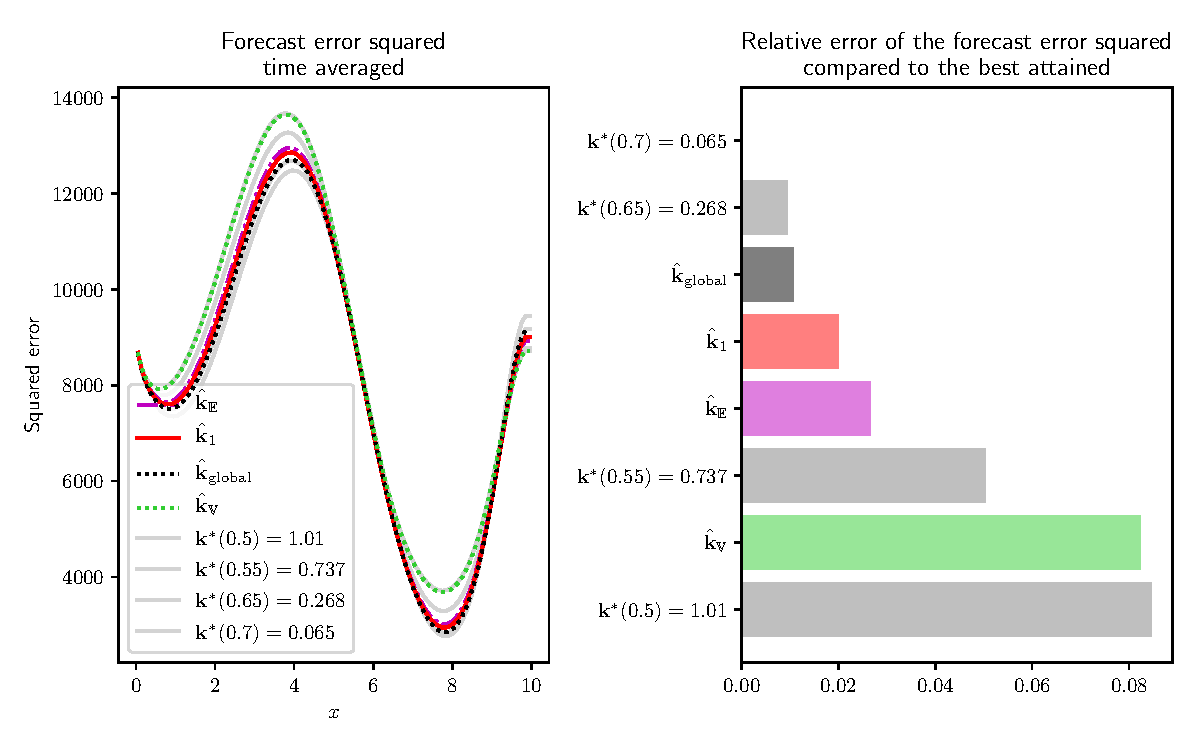
\includegraphics[width=\onehalfcolumn]{Figures/L2_full_rel.pdf}
\caption{Squared forecast error for the shallow water case, depending on the calibrated parameter. The left figure shows the squared error time-averaged as a function of the spatial coordinate $x$, while the right barplot shows the relative change of the mean forecast error, averaged over time and space, taken w.r.t.\ to the best attained performance for $\mathbf{k}^*(0.7)$}
\label{fig:forecast_squared_error}
\end{figure*}

We can see that the mean forecast error squared, on the right side, averaged over time and space is the smallest for the conditional minimisers $\kest^*(0.7)$ and $\kest^*(0.65)$, then $\kest_{\mathrm{global}}$, while $\kest_{1.0}$ performs slightly better than $\hatkmean$.


It may seem surprising that some parameters calibrated without a robustness aspect perform better than $\kest_1$ and $\hatkmean$, but their performances are largely dependent on the choice of $\mathbf{u}$ and their associated conditional minimisers. Good forecasts can be achieved as well as bad ones, as shown for $\mathbf{u}=0.5$, that leads to bad forecasts.

One issue with the squared forecast error is that it will penalize strongly the forecasts that present high variability with respect to the environmental conditions.
A way to deal with this is to use another metric, that takes the probabilistic nature of the forecasts into account.


\subsubsection{Continuous Ranked Probability Score}
Given the random variables $\mathcal{M}_{\mathrm{pred}}(\kest, \mathbf{U})$ and $\mathcal{M}_{\mathrm{pred}}^o(\mathbf{U})$, representing the probabilistic forecast and the probabilistic observations, we can define the cumulative distribution functions (CDF) $F_{\mathrm{pred}}(\cdot, \kest)$ and $F^o_{\mathrm{pred}}(\cdot)$
The Continuous ranked probability score (CRPS) measures the squared difference between the predicted CDF $F_{\mathrm{pred}}$ using a calibrated value, and the CDF of the observations $F_{\mathrm{pred}}^o$. 
\begin{equation}
\label{eq:def_crps}
\mathrm{CRPS}(\mathbf{k}) = \int_{\mathbb{R}} (F_{\mathrm{pred}}(\xi,\mathbf{k}) - F^o_{\mathrm{pred}}(\xi))^2 \,\mathrm{d}\xi
\end{equation}

\begin{figure}[!h]
  \centering
  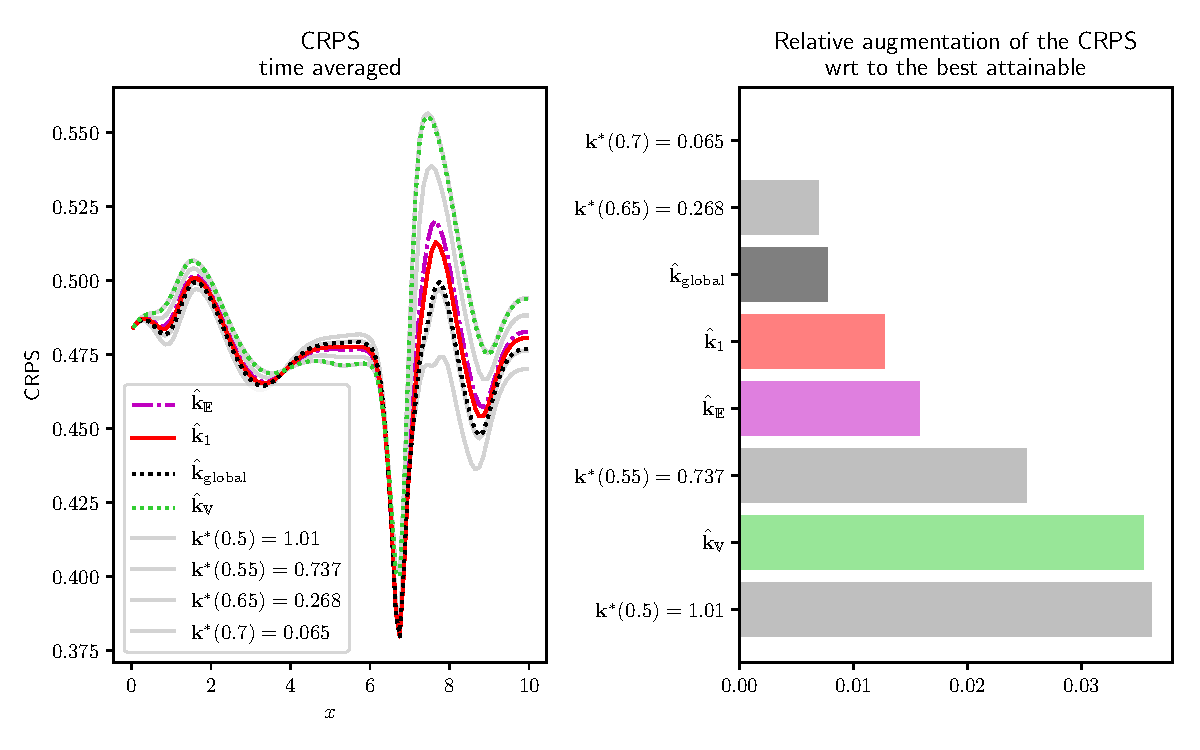
\includegraphics[width=\onehalfcolumn]{Figures/CRPS_full_rel}
  \caption{CRPS computed for different calibrated parameters for the shallow water case. The left figure shows the CRPS time-averaged as a function of the spatial coordinate $x$, and the right figure shows the relative change of the CRPS averaged over time and space, taken with respect to the best attained CRPS for $\mathbf{k}^*(0.7)$}
\label{fig:forecast_crps}
\end{figure}

The left plot of Figure~\ref{fig:forecast_crps} shows the CRPS averaged over time, where $x$ denotes the spatial coordinate and the right plot shows the value of the CRPS averaged over time and space. The difference between the squared forecast error and the CRPS is apparent when comparing the general trends shared by the different calibrated parameters. According to the squared error, the sea water height of the physical region $x=4$ is not well predicted, while around $x=8$, the predictions are better. On the other hand, according to the CRPS, the region around $x=8$ provide worse forecasts than when $x=4$ and $x=7$. Given the properties of the two metrics,  we can conclude that the region around $x=4$ presents a lot of variability with respect to $\mathbf{u}$, for both the true model and the numerical one. However, for $x \approx 8$, there is a lot less variability, as the low squared error indicates, but probably a higher bias, due to the systematic errors between the truth and the numerical model.


The numerical evaluations of the CRPS for different parameters show the same order of performances observed for the squared error: the calibrated parameters that present the best performances for forecasts according to those two metrics are $\kest^*(0.7)$, $\kest^*(0.65)$ which is very similar to $\kest_{\mathrm{global}}$, and then $\kest_1$, and $\hatkmean$.
This presupposes to know which $\mathbf{u}$ to choose for the conditional minimisation, thus having a strong insight on the value of the parameters in the first place.

% ----------------------------------------------------------------------
\section*{Conclusion}

In this paper, we dealt with a problem of robust calibration, or in other terms, the robust minimisation of an objective function. To adress this issue, we proposed a new set of robust estimators: the family of the \RRE{} (Relative-regret estimators), and compared it in a forecast context to some other robust estimators, for the calibration of the bottom friction of a shallow water model.

Our approach is based on the will to be as close as possible to the conditional minimisers with high probability. At a level $p$, in addition to the estimation, we have the relaxation coefficient $\alpha_p$ that bounds with probability $p$ the relative error of the cost function. This helps us to assess the robustness properties of the proposed estimation.  

Except for simple analytical examples, the exact evaluation of a member of the \RRE{} is very expensive computer-wise, not to say impossible. Some bottlenecks appear: the computations of the conditional minimisers $\mathbf{k}^*(\mathbf{u})$ and the minimum $J^*(\mathbf{u})$, that require very local exploration of $\Kspace$ for every $\mathbf{u}$; and the computations of the probability of overshooting a given bound that depends on $J^*(\mathbf{u})$ (analogous to a probability of failure), task that requires an efficient exploration of the whole sample space $\Uspace$.

For the calibration of the shallow water model presented in Section~\ref{sec:SWE_application}, we chose to construct a response surface based on Gaussian processes, which is then used for the extensive computations. This construction is first based on an initial design, that is enriched to better capture the locus of the conditional minimisers using the PEI criterion introduced in~\cite{ginsbourger_bayesian_2014}. 

Comparing the performances of the different estimates in a forecast context, one can see that for the two metrics introduced in Section~\ref{sec:SWE_application}, $\kest_1$ performs better than $\hatkmean$, but is sometimes outperformed by ``non-robust'' solutions. Those require some additional knowledge about the environmental conditions, and did not present some robust properties during the calibration phase.

Practically speaking, the estimation of those quantities is very crude, so the computational cost may be very expensive. As perspective, specific strategies have to be created, based for instance on sequential design of computer experiments using Gaussian processes, to diminish the amount of runs needed of the numerical model. Ideally, one would want to develop an acquisition criterion, that makes the balance between the minimisation of a well-chosen probability of failure, and the exploration around the conditional minimisers.
Finally, the models upon which this calibration procedure have been applied are very simplistic. We plan in the future to apply this to the robust calibration of the bottom friction of a realistic model of the ocean.
% \victor{À faire à la fin}
% This paper deals with the problem of robust calibration of a computer code in the presence of uncertain inputs. 

% Our contribution consists in introducing a new criterion of robustness, based on the distribution of the minimisers. More specifically, this estimate is bounding the ratio between the cost function and its conditional minimum.
% Experimental results show that this new estimate is able to make a compromise between the minimum of the expected value and the minimum of the variance, will also giving the range of the ratio evoked above.

% From a practical perspective, this estimation is very expensive: each evaluation of $\mathbf{k}^*$ requires an optimisation procedure. The distribution of the conditional minimisers is then very complicated to compute.
% In addition to that, in order to relax the constraint, the cost function must also be evaluated in the vicinity of the conditional minimisers. Computing precisely this estimate is then intractable if each run of the underlying model is expensive (longer than a couple of seconds).


% A solution to explore is the use of surrogate models. Based on an initial design of experiment, the (expensive) cost function is replaced by a function, that is cheap to evaluate.
% For instance,~\cite{ginsbourger_bayesian_2014}
% uses Gaussian Process regression and sequential methods to explore the conditional minimisers.

% Finally, the adaptibility of this method has to be studied in a higher dimensional setting. High-dimensional density estimation is a challenge in itself, but is necessary in order to tackle more realistic applications.
% \appendix
% \section{}    %% Appendix A

%% If you have bibdatabase file and want bibtex to generate the
%% bibitems, please use
%%
%%  \bibliographystyle{elsarticle-num-names} 
%%  \bibliography{<your bibdatabase>}

%% else use the following coding to input the bibitems directly in the
%% TeX file.

\bibliographystyle{model1-num-names} 
\bibliography{biblio_file}

\end{document}

\endinput
%%
%% End of file `elsarticle-template-num-names.tex'.

%%% Local Variables:
%%% mode: latex
%%% TeX-master: t
%%% End:
